\documentclass[11pt]{article}
\usepackage[T1]{fontenc}
\usepackage{mathpazo}
\usepackage[margin=1in]{geometry}
\usepackage{amsmath,amssymb,amsthm,mathtools}
\usepackage{mathrsfs}
\usepackage{microtype}
\usepackage[numbers,sort&compress]{natbib}
\usepackage{xcolor}
\usepackage{tikz}
\usetikzlibrary{arrows.meta,positioning,calc}
\usepackage{hyperref}
\urlstyle{same}
\hypersetup{
  colorlinks=true,
  linkcolor=blue!55!black,
  citecolor=blue!55!black,
  urlcolor=blue!55!black,
  pdftitle={The unique threshold bound state of the SU(N) BFSS model},
  pdfauthor={OpenAI}
}
\input{glyphtounicode}
\input{glyphtounicode-cmex}
\pdfglyphtounicode{mapsto}{007C}
\pdfglyphtounicode{arrowhookleft}{02D3}
\pdfgentounicode=1
\pdftrailerid{}
\numberwithin{equation}{section}
\newtheorem{theorem}{Theorem}[section]
\newtheorem{proposition}[theorem]{Proposition}
\newtheorem{lemma}[theorem]{Lemma}
\newtheorem{corollary}[theorem]{Corollary}
\theoremstyle{definition}
\newtheorem{definition}[theorem]{Definition}
\theoremstyle{remark}
\newtheorem{remark}[theorem]{Remark}
\DeclareMathOperator{\Tr}{Tr}
\DeclareMathOperator{\ad}{ad}
\DeclareMathOperator{\Spin}{Spin}
\DeclareMathOperator{\SU}{SU}
\DeclareMathOperator{\U}{U}
\DeclareMathOperator{\diag}{diag}
\DeclareMathOperator{\supp}{supp}
\DeclareMathOperator{\dist}{dist}
\DeclareMathOperator{\Ker}{ker}
\DeclareMathOperator{\Ran}{ran}
\newcommand{\R}{\mathbb R}
\newcommand{\C}{\mathbb C}
\newcommand{\N}{\mathbb N}
\newcommand{\cH}{\mathcal H}
\newcommand{\cK}{\mathcal K}
\newcommand{\Id}{\mathrm{Id}}
\newcommand{\dd}{\mathrm d}
\newcommand{\ii}{\mathrm i}
\newcommand{\norm}[1]{\left\lVert #1\right\rVert}
\newcommand{\abs}[1]{\left\lvert #1\right\rvert}
\newcommand{\ip}[2]{\left\langle #1,#2\right\rangle}
\setlength{\emergencystretch}{1em}
\setcounter{tocdepth}{1}
\title{The unique threshold bound state of\texorpdfstring{\\}{ }the \(\SU(N)\) BFSS model}
\author{OpenAI}
\date{September 24, 2026}

\begin{document}
\maketitle
\begin{abstract}
For every finite \(N\ge2\), we prove that undeformed \(\SU(N)\) BFSS matrix
quantum mechanics has exactly one normalizable zero-energy state after
removing the center of mass. This establishes the threshold-bound-state
conjecture.
\end{abstract}

\tableofcontents
\clearpage

\section{Introduction}
\label{sec:introduction}

Supersymmetric matrix quantum mechanics appears in the regularization of
supermembranes~\cite[Section~3]{DeWitHoppeNicolai1988} and in the
matrix-theory conjecture of Banks, Fischler, Shenker, and
Susskind~\cite{BFSS1997}. The model studied here describes nine Hermitian
matrices and their fermionic partners. Its commuting configurations form
noncompact flat directions.
The D0-brane bound-state prediction of Witten~\cite[Section~4.2]{Witten1996BoundStates},
subsequently central to matrix theory, is that after removing the free
center of mass every finite matrix size has exactly one normalizable
state of zero energy. We prove this threshold-bound-state conjecture for the
\(\SU(N)\) model on its full configuration space.
In the matrix-theory interpretation, this relative bound state supplies
the internal state of a single supergraviton carrying \(N\) units of
longitudinal momentum~\cite[Section~5]{BFSS1997}.
The continuous spectrum starts at zero~\cite{DeWitLuscherNicolai1989},
so the proposed eigenstate lies at its threshold rather than below a
gapped continuum.

\subsection{The operator and the result}
\label{sec:model}

Fix an integer \(N\ge2\) and put \(d_N=N^2-1\).
Choose a traceless Hermitian basis \(T_A\), \(1\le A\le d_N\), with
\[
\Tr(T_AT_B)=\delta_{AB},\qquad
T_AT_B-T_BT_A=\ii f_{ABC}T_C.
\]
Repeated indices are summed unless stated otherwise.
The bosonic coordinates and momenta are
\[
X_i=x_i^AT_A,\qquad p_i^A=-\ii\frac{\partial}{\partial x_i^A},
\qquad 1\le i\le9.
\]
Let \(\mathcal F_N\) be an irreducible complex Clifford module with
self-adjoint generators \(\theta_\alpha^A\), \(1\le\alpha\le16\), satisfying
\[
\{\theta_\alpha^A,\theta_\beta^B\}
  =\delta_{\alpha\beta}\delta_{AB}.
\]
Choose real symmetric \(16\times16\) matrices \(\gamma^i\) with
\(\{\gamma^i,\gamma^j\}=2\delta_{ij}\Id\), and set
\(\gamma^{ij}=[\gamma^i,\gamma^j]/2\), where the bracket in this formula
is the ordinary matrix commutator. The sixteen supercharges on smooth
compactly supported functions are
\begin{equation}
Q_\alpha
 =p_i^A\gamma^i_{\alpha\beta}\theta_\beta^A
 +\frac12 f_{ABC}x_i^Bx_j^C
       \gamma^{ij}_{\alpha\beta}\theta_\beta^A.
\label{eq:model-charge}
\end{equation}
The physical Hilbert space is
\[
\mathscr H_N
 =\bigl[L^2(\R^{9d_N})\otimes\mathcal F_N\bigr]^{\SU(N)},
\]
with the simultaneous adjoint action on bosons and fermions. Let \(H_N\)
be the nonnegative self-adjoint operator associated with the closure of
the quadratic form
\begin{equation}
q_N(\Psi)=\frac1{16}\sum_{\alpha=1}^{16}\norm{Q_\alpha\Psi}^2
\label{eq:model-form}
\end{equation}
on the gauge-invariant compactly supported smooth core. This fixes the
coupling and the operator domain used throughout the paper.
We use the exterior grading for the polarization
$T=\gamma^1\gamma^2\gamma^3$, declaring its empty vector even and
choosing that vector to minimize $\ii\theta^tT\theta/2$.
Section~\ref{sec:algebra} describes the associated symmetry actions.

\begin{theorem}\label{thm:main}
For every integer \(N\ge2\),
\[
\dim\Ker H_N=1.
\]
The kernel consists of \(\Spin(9)\)-invariant states and is even in the
fermion grading just specified.
\end{theorem}

All square integrability in Theorem~\ref{thm:main} is on the whole
space \(\R^{9d_N}\). Constants in the proof may depend on the fixed
integer \(N\). The free \(\U(1)\) center-of-mass coordinates do not occur
in \(\mathscr H_N\).

\subsection{History and the analytic issue}

The supersymmetric index counts even and odd zero modes with opposite
signs~\cite{Witten1982Index}. In the present noncompact problem,
contributions from infinity are essential. Yi~\cite{Yi1997} computed the
$\SU(2)$ bulk term and proposed a free-particle argument for its boundary correction;
Sethi--Stern~\cite{SethiStern1998} obtained the two-particle index by
including its boundary term. Moore--Nekrasov--Shatashvili~\cite{MNS2000}
computed the matrix integrals entering the principal contribution.
Green--Gutperle~\cite[Section~5]{GreenGutperle1998} argued that corrections
from free identical clusters account for the divisor sum, assuming the
free-cluster boundary prescription extends to general $N$.
Konechny~\cite[Sections~3 and~5]{Konechny1999} derived a free leading
asymptotic Hamiltonian and used it to conclude that the full $\SU(N)$
index equals one. His expansion assumes that the eigenvalue differences
of one diagonalized matrix grow at the same order. Our proof will
control also the degenerating and nested cluster regions through
explicit norm estimates.

A signed count becomes a dimension count once odd normalizable ground
states are excluded. Sethi--Stern~\cite[Sections~3.2 and~4.2]{SethiStern2000} proved rotational
invariance of normalizable ground states of ten-dimensional reductions.
Hasler--Hoppe~\cite[Theorem~1(a) and Lemma~2(c)]{HaslerHoppe2002} gave a direct
rotation anticommutator and cutoff proof on the full physical Hilbert
space. In the fermion representation used here, singletness implies
even parity. Section~\ref{sec:algebra} reproduces these arguments in
our normalization and fixes the closed operator domains. The recent
lectures of Lin~\cite[Section~3.1]{Lin2026v3} describe the finite-$N$ spectral picture
and distinguish the two-particle uniqueness consequence from the general
conjecture.

Asymptotic wavefunction analysis supplies a second important line of
work. Halpern--Schwartz~\cite{HalpernSchwartz1998} developed a generalized
Born--Oppenheimer search for $\SU(2)$ candidates. Graf--Hoppe~\cite{GrafHoppe1998}
computed the leading and subleading $\SU(2)$ asymptotics, and
Fr\"ohlich--Graf--Hasler--Hoppe--Yau~\cite[Section~3]{FroehlichEtAl2000} classified
the corresponding invariant formal supercharge expansions at infinity. For general rank, Hasler--Hoppe~\cite[pp.~2--5]{HaslerHoppeFactorization2002}
conjugated the charge by the slice density, projected onto its transverse
oscillator ground state, and obtained the leading free Cartan charge.
Their cancellation of the gauge-spin and density terms is a direct
predecessor of the computation in Section~\ref{fast:section}.
Lin--Yin~\cite[Sections~3.2 and~4]{LinYin2015} developed a recursive cluster-factorization
proposal and its first inverse-oscillator correction. These asymptotic
constructions motivate the local objects used below; a global
normalizable state additionally requires control of every cluster scale
and of all limiting norm.

Mass deformation offers a finite count from which to approach that
global problem. Porrati--Rozenberg~\cite{PorratiRozenberg1998} formulated
a deformation criterion with explicit normalizability requirements on
weighted representatives. Kac--Smilga~\cite{KacSmilga2000} counted
mass-deformed vacua and identified persistence of normalizability at
zero mass as the remaining hypothesis. We use the completely confining
plane-wave deformation of Berenstein--Maldacena--Nastase~\cite{BMN2002}.
Its classical zero orbits are indexed by integer partitions of $N$.
Dasgupta--Sheikh-Jabbari--Van Raamsdonk~\cite{DasguptaSheikhJabbariVanRaamsdonk2002}
computed the quadratic fluctuation spectra around the reducible as well as
irreducible vacua. Section~\ref{sec:massive-index} rederives these
frequencies and proves the stabilizer, domain, and norm-exhaustion
statements needed for the index of our specified invariant charge.
Chang's refined BMN index~\cite[Section~2.2]{Chang2025} also records signed
contributions from states with nonzero angular momentum. The count below
is the Fredholm index of a real charge on a specified invariant subspace.

The operator domain must remain fixed throughout this comparison.
Boulton--Garc\'ia del Moral--Restuccia~\cite[Sections~5--6]{Boulton2021}
establish existence and uniqueness for a valley boundary-value problem
with admissible prescribed trace. The realization with zero boundary trace has trivial
kernel, while the solutions with prescribed nonzero trace need not be
killed by the supercharges. That problem
therefore concerns a different realization from
\eqref{eq:model-form}.

The task addressed here is the passage from a massive Fredholm count
to the complete $L^2$ kernel of the undeformed full-space operator.
The local oscillator projections and fast-inverse corrections are
proved with graph-norm bounds near arbitrary proper clusters.
An exterior estimate, established simultaneously with the kernel
statement, excludes norm at intermediate internal scales. Together
with massive confinement, it accounts for every limiting norm and
inner product. This is the information that permits the final
unsigned dimension comparison.

\subsection{The proof and its compactness mechanism}

Write $\mathcal K_n=\Ker H_n$ and set $\mathcal K_1=\C$. The proof compares
$\mathcal K_N$ with a massive problem whose index is the partition number
$p(N)$, the number of unordered integer partitions of $N$. Two different
uses of partitions enter this comparison. At small coupling, they label
the massive classical vacuum orbits. In the limiting cluster decomposition, a proper
partition $C=(n_1,\ldots,n_k)$, $k\ge2$, specifies the sizes of separated
commuting blocks. Their distinct centers $c_\alpha\in\R^9$ satisfy
$\sum_\alpha n_\alpha c_\alpha=0$. A \emph{cluster profile} is a
wavefunction of these relative centers, with their fermions and with
values in $\bigotimes_\alpha\mathcal K_{n_\alpha}$.

For the dimension comparison, we study profiles of normalized massive
states whose charge norms tend to zero; we call these null profiles.
The proper partitions will contribute $p(N)-1$ lines of null profiles, while
a full-collapse profile takes values in $\mathcal K_N$. The comparison
uses norm-preserving extraction for existence, and recovery of prescribed
profiles together with a massive spectral gap for uniqueness.

\paragraph{The massive count.}
We write $D_v(h,m)$ for the deformed charge paired with a real unit
spinor $v$, where $h>0$ multiplies the commutator term and $m\ge0$
multiplies the linear mass term. Thus
$D_v(1,0)=\sum_\alpha v_\alpha Q_\alpha$.
Section~\ref{sec:algebra} chooses a spinor $u$ and a connected fixing
torus $G$ so that, on gauge and $G$ invariants,
\[
 D_u(h,m)^2\ge\frac23\mathcal H(h,m),
\]
where $\mathcal H$ is the averaged squared charge. At fixed positive mass,
the restricted charge is Fredholm. Section~\ref{sec:massive-index}
computes its index as $p(N)$ in the limit $h\downarrow0$ and proves
constancy for all $h>0$.

We then study $h\to\infty$ at mass one. The unitary change of variables
$y=h^{1/3}x$ sends $D_v(h,1)$ to
$h^{1/3}D_v(1,h^{-2/3})$, so this limit is a massless limit at the original
coupling. Internal block states shrink on the physical scale $h^{-1/3}$,
while their relative centers remain on scale one.

\paragraph{Local profiles and their equations.}
Near distinct block centers, a spectral slice separates the block
variables $b$ from the off-block variables. After rescaling the latter,
Section~\ref{fast:section} gives the exact decomposition
\[
 D_v(h,m)=\sqrt h\,E_v(b)+D_v^s(h,m)+R_v.
\]
Here $E_v$ acts on the transverse variables and their fermions,
$D_v^s$ is the charge of the block variables, and $R_v$ collects the
remaining slice terms. On the fast space fixed
by the block-center gauge torus, $E_v$ has an even one-dimensional
kernel and a local oscillator gap. A first-order estimate then forces
bounded graph-norm sequences onto this line. In the scalar-block limit,
compressing the charge onto this line gives the ordinary slow charge:
the gauge-spin term cancels the derivative of
the slice density.

To pass the charge equation to a profile, we need more than concentration
of the state. Section~\ref{lift:section} constructs test states whose
charge outputs converge in norm. A correction obtained from the reduced
fast inverse cancels the perpendicular charge output of the leading
oscillator product. Duality then identifies the center equation of each
profile. Fixed physical cutoffs and $L^2$ concentration make these
constructions available without moment bounds on the internal kernels.

\paragraph{Capturing every concentration scale.}
Local profiles leave a possible loss of norm between the internal scale
$h^{-1/3}$ and a vanishing physical radius. Section~\ref{sec:profiles}
excludes that loss by proving, simultaneously with Theorem~\ref{thm:main},
the exterior estimate
\begin{equation}
 \norm{rD_u(h,0)F}\ge c_N\norm F,
 \qquad
 \supp F\subset\{h^{1/3}r>R_N\},\qquad r=|x|.
 \label{eq:intro-exterior}
\end{equation}
It applies to compactly supported gauge-invariant vectors in the charge
graph domain, without a rotation restriction. The
smaller-block estimates make proper-cluster profiles account for all
norm on a compact annulus. Their center spaces have dimensions
$9(k-1)\ge9$, so the Euclidean Hardy inequality gives the exterior
estimate at the current size. Only after this step do we extract the
whole-block profile at the origin. The induction therefore uses no
prior existence or dimension statement for $\mathcal K_N$.

Section~\ref{sec:counting} proves a separate massive annular estimate
that prevents escape to infinity. The resulting decomposition preserves
all limiting norms and inner products. Each proper null profile has the
unique even massive center-oscillator vacuum as its center factor. Induction
on the internal blocks and the permutation symmetries then give one
line for each of the $p(N)-1$ proper partitions. Every null profile is even:
Proposition~\ref{prop:singlet-parity} proves this for $\mathcal K_N$
before its dimension is known. Consequently odd massive states have a
uniform charge gap at large $h$. Spectral pairing gives the same gap
on the even complement of the massive kernel, and the index becomes
the exact massive dimension $p(N)$. Extracting these $p(N)$ directions
forces a nonzero whole-block profile. Conversely, recovering any finite
orthonormal whole-block list along with the $p(N)-1$ proper lines and projecting
through the gap bounds that list by one. This closes the induction.

Figure~\ref{fig:induction} records this order of dependencies.
\begin{figure}[!htbp]
\centering
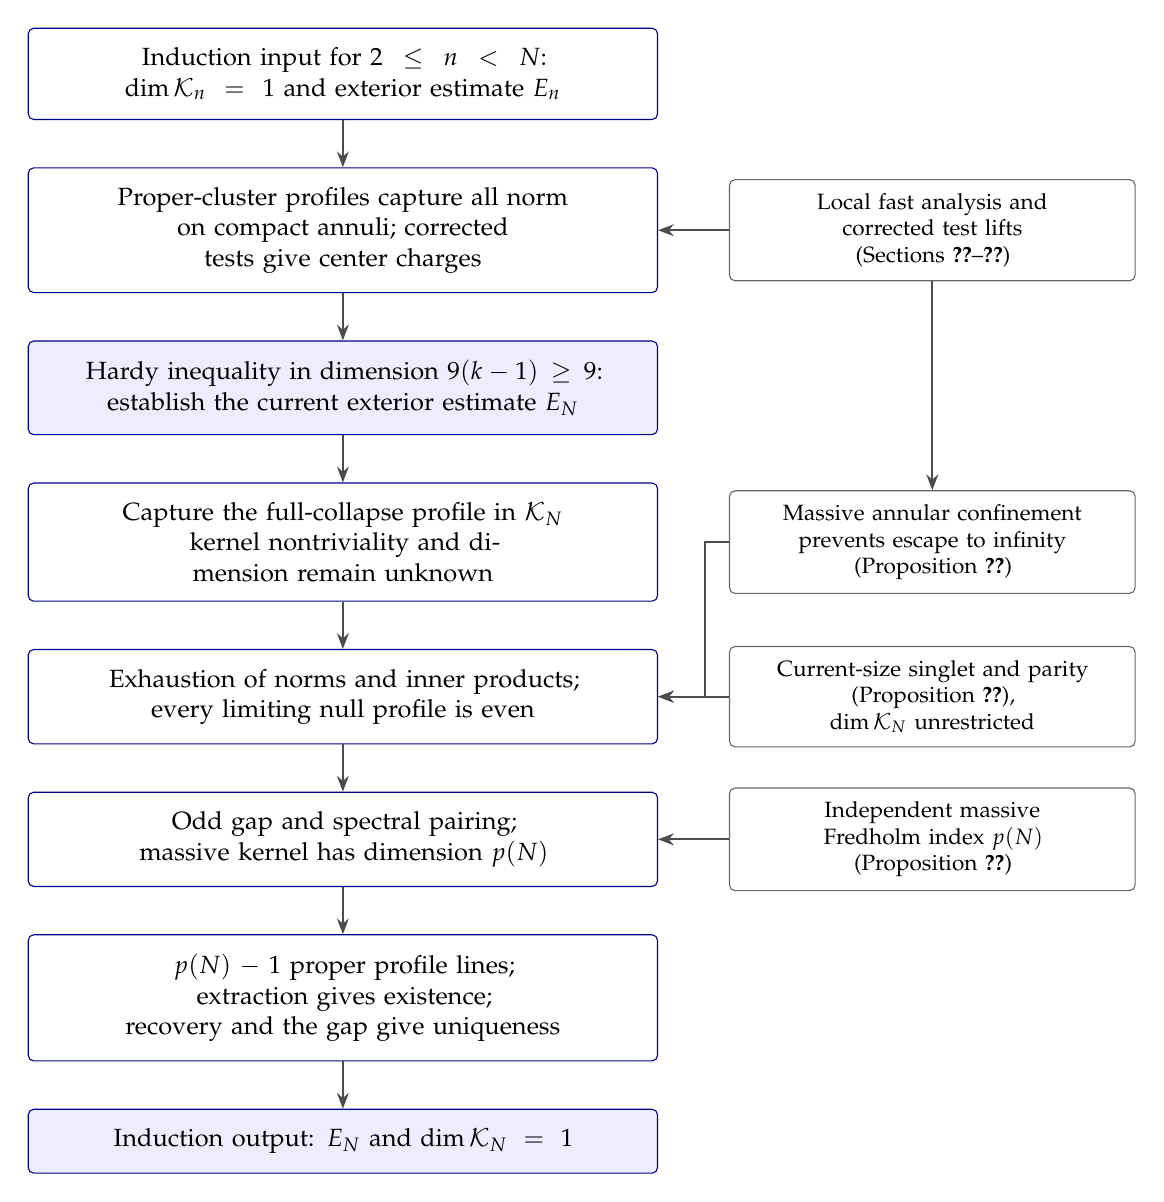
\begin{tikzpicture}[
  box/.style={draw=blue!55!black,rounded corners=2pt,align=center,
    text width=7.5cm,inner sep=7pt,font=\small},
  side/.style={box,text width=4.8cm,draw=black!60,
    inner sep=5pt,font=\footnotesize},
  flow/.style={-{Stealth[length=2mm]},thick,draw=black!70},
  node distance=6mm and 9mm]
\node[box] (input) {Induction input for $2\le n<N$:\\
  $\dim\mathcal K_n=1$ and exterior estimate $E_n$};
\node[box,below=of input] (proper) {Proper-cluster profiles capture all norm\\
  on compact annuli; corrected tests give center charges};
\node[box,below=of proper,fill=blue!7] (ext) {Hardy inequality in dimension $9(k-1)\ge9$:\\
  establish the current exterior estimate $E_N$};
\node[box,below=of ext] (collapse) {Capture the full-collapse profile in $\mathcal K_N$\\
  kernel nontriviality and dimension remain unknown};
\node[box,below=of collapse] (exhaust) {Exhaustion of norms and inner products;\\
  every limiting null profile is even};
\node[box,below=of exhaust] (gap) {Odd gap and spectral pairing;\\
  massive kernel has dimension $p(N)$};
\node[box,below=of gap] (count) {$p(N)-1$ proper profile lines;\\
  extraction gives existence;\\recovery and the gap give uniqueness};
\node[box,below=of count,fill=blue!7] (output) {Induction output: $E_N$ and $\dim\mathcal K_N=1$};
\node[side,right=of proper] (local) {Local fast analysis and\\corrected test lifts\\
  (Sections~\ref{fast:section}--\ref{lift:section})};
\node[side,right=of collapse] (tight) {Massive annular confinement\\
  prevents escape to infinity\\(Proposition~\ref{prop:massive-tightness})};
\node[side,right=of exhaust] (parity) {Current-size singlet and parity\\
  (Proposition~\ref{prop:singlet-parity}),\\$\dim\mathcal K_N$ unrestricted};
\node[side,right=of gap] (index) {Independent massive\\Fredholm index $p(N)$\\
  (Proposition~\ref{prop:massive-index})};
\foreach \a/\b in {input/proper,proper/ext,ext/collapse,collapse/exhaust,
  exhaust/gap,gap/count,count/output}\draw[flow] (\a)--(\b);
\draw[flow] (local)--(proper);
\draw[flow] (local)--(tight);
\draw[flow] (tight.west)--++(-0.3,0)|-(exhaust.east);
\draw[flow] (parity)--(exhaust);
\draw[flow] (index)--(gap);
\end{tikzpicture}
\caption{The simultaneous induction. Here $\mathcal K_n=\ker H_n$ and
$E_n$ is Proposition~\ref{prop:exterior-estimate} at size $n$.
The highlighted exterior step is completed before full collapse is
used. Massive confinement follows independently from the local
growing-mass estimates, and the index is computed independently at
small coupling. At $N=2$ all proper blocks are scalar, so the induction
input is empty.}
\label{fig:induction}
\end{figure}

\clearpage

\section{The charge algebra, domains, and rotational invariance}
\label{sec:algebra}

We establish the operator framework needed for the index and limiting
arguments: closed charge domains, a charge coercive on a chosen space
of torus invariants, and even rotationally invariant undeformed kernel
vectors.

We use the real Euclidean space \(\mathfrak k\) of traceless Hermitian
matrices, with scalar product \(\Tr(XY)\) and real Lie bracket
\([X,Y]=(XY-YX)/\ii\). Thus \(\ad(X)\) is a real skew matrix on
\(\mathfrak k\). Uppercase Roman indices denote an orthonormal color
basis and Greek indices denote spinor components;
\(i,j=1,\ldots,9\), \(a,b,c=1,2,3\), and \(d=4,\ldots,9\) are spatial
indices. For \(w\in\R^{16}\) and \(z\in\mathfrak k\), write
\(\theta(w)\cdot z=\sum_{\alpha,A}\theta_\alpha^A w_\alpha z^A\).
All Clifford tensor products are graded tensor products.

Set
\[
 T=\gamma^1\gamma^2\gamma^3,\qquad
 s_a=2,\quad s_d=-1,
 \qquad A_i(v)=\gamma^i v,\quad
 B_{ij}(v)=-\gamma^{ij}v,\quad L_i(v)=s_i\gamma^iTv.
\]
Here \(T^t=-T\), \(T^2=-\Id\), and \(T\) commutes with the first
three gamma matrices and anticommutes with the other six. For a unit
real spinor \(v\), coupling \(h>0\), and mass \(m\geq0\), define
\begin{equation}
\label{eq:deformed-charge}
\begin{aligned}
 D_v(h,m)&=\sum_i\theta(A_i(v))\cdot p_i
 +h\sum_{i<j}\theta(B_{ij}(v))\cdot[x_i,x_j]
 +m\sum_i\theta(L_i(v))\cdot x_i,\\
 \cH(h,m)&=\frac1{16}\sum_{\nu=1}^{16}D_{v_\nu}(h,m)^2.
\end{aligned}
\end{equation}
The second expression initially denotes a quadratic form on the
gauge-invariant smooth compactly supported core; \((v_\nu)\) is any
orthonormal real spin basis. Its closure will have the same notation.
The minus sign in \(B_{ij}\) is the transpose sign in
\((\gamma^{ij})^t=-\gamma^{ij}\), so \(D_v(1,0)\) is exactly the
linear combination of the charges in \eqref{eq:model-charge} with
coefficients \(v\).

For a real skew spatial matrix \(F\), use the rotation conventions
\begin{equation}
\label{alg:rotation-generator}
 S(F)=\frac14\sum_{i,j}F_{ij}\gamma^i\gamma^j,
 \qquad
 J(F)=p\cdot Fx+\frac{\ii}{2}\theta^t S(F)\theta.
\end{equation}
The color identity in the second term is implicit. In particular,
\(J\) includes both orbital and spin rotations. Gauge invariance means
equivariance of the Clifford-valued function, rather than invariance
of its scalar coordinate dependence alone. Infinitesimally this gives
\begin{equation}
\label{alg:gauge-generator}
 p\cdot\ad(w)x=-\frac{\ii}{2}\theta^t\ad(w)\theta
 \quad\text{on gauge-invariant functions},\qquad w\in\mathfrak k.
\end{equation}

\begin{proposition}[Square of a charge]
\label{prop:square}
On the gauge-invariant core,
\begin{equation}
\label{eq:square}
\begin{aligned}
 \cH(h,m)&=\frac12p^2+U_{h,m}
   +\frac{\ii}{2}\theta^t\left(\frac32mT-hK_j\gamma^j\right)\theta,
       \qquad K_j=\ad(x_j),\\
 2U_{h,m}&=\sum_{\mathrm{cyc}}
       \abs{h[x_a,x_b]-2mx_c}^2
       +h^2\sum_{\substack{i<j\\j>3}}\abs{[x_i,x_j]}^2
       +m^2\sum_{d=4}^9\abs{x_d}^2,\\
 D_v(h,m)^2&=\cH(h,m)+mJ(R(v)),
       \qquad R(v)_{ij}=s_jv^t\gamma^i\gamma^jTv.
\end{aligned}
\end{equation}
The cyclic sum uses \((a,b,c)=(1,2,3),(2,3,1),(3,1,2)\).
The matrix \(R(v)\) is skew, preserves \(\R^3\oplus\R^6\), and has
zero spin-basis average. The same formulas hold for an orthogonal
direct sum of compact color algebras and abelian color spaces.
\end{proposition}

\begin{proof}
\emph{The massless square.}
We first compute the kinetic and commutator contributions, including
the gauge cancellation. For a strictly increasing multi-index \(I\), let \(\gamma^I\) denote
the corresponding ordered gamma product. The products of ranks zero
through four form an orthogonal basis of the real \(16\)-by-\(16\)
matrices, for the trace scalar product. Indeed there are
\(1+9+36+84+126=256\) of them. Every nonconstant product of at most
eight distinct gammas is traceless: conjugation by a gamma outside the
product changes its sign for odd rank, and conjugation by a gamma
inside changes its sign for positive even rank. This also proves
orthogonality. The symmetric products have ranks zero, one, and four;
the skew products have ranks two and three.

Put \(\operatorname{sym}M=(M+M^t)/2\) and
\(\operatorname{skew}M=(M-M^t)/2\). The identity needed for the Yukawa
term is
\begin{equation}
\label{alg:spin-identity}
 \sum_i\operatorname{sym}\bigl((\gamma^iv)(\gamma^{ij}v)^t\bigr)
 =\frac12(v^t\gamma^jv)\Id-\frac12\gamma^j.
\end{equation}
To check it, test its left side against a symmetric monomial
\(M=\gamma^I\) of rank \(r\). Since
\(\sum_i\gamma^iM\gamma^i=(-1)^r(9-2r)M\), its trace pairing is
\[
 \bigl((-1)^r(9-2r)-1\bigr)v^tM\gamma^jv.
\]
For \(r=0,1,4\), this is respectively
\(8v^t\gamma^jv\), \(-8\delta_{Ij}\), and zero, which are precisely
the pairings with the right side of \eqref{alg:spin-identity}.

The CAR give \(\theta(w)^2=\abs{w}^2/2\). They therefore give the
kinetic term \(p^2/2\). The square of the bracket multiplier is
\(h^2\sum_{i<j}\abs{[x_i,x_j]}^2/2\): its possible remaining
four-form term is proportional to the alternating sum of
\(\ip{[x_i,x_j]}{[x_k,x_l]}\), and vanishes by invariance of the
color scalar product and the Jacobi identity.

The scalar, first-order part of the kinetic--bracket anticommutator is
\(h(v^t\gamma^jv)p\cdot K_jx\). In differentiating the bracket
coefficient with respect to \(x_i^A\), its component of color \(B\),
divided by \(h\), has spin coefficient
\(\sum_j(K_j)_{BA}\gamma^{ij}v\). Since \(K_j\) is skew in color,
its contraction with the kinetic Clifford multiplier selects the
symmetric spin matrix in \eqref{alg:spin-identity}. Consequently the
differentiated part is
\[
 -\frac{\ii h}{2}\theta^tK_j\gamma^j\theta
 +\frac{\ii h}{2}(v^t\gamma^jv)\theta^tK_j\theta.
\]
The second term cancels the first-order term by
\eqref{alg:gauge-generator}. This proves all the massless terms in
\eqref{eq:square}.

\smallskip\noindent\emph{The mass and rotation terms.}
The vectors \(L_i(v)\) have Gram matrix
\(\ip{L_i(v)}{L_j(v)}=s_i^2\delta_{ij}\). The bracket--mass
anticommutator is a scalar multiplier. Its color contractions are
alternating in three distinct spatial indices. Their spin coefficient
is proportional to
\[
 (s_i+s_j+s_k)v^t\gamma^i\gamma^j\gamma^kTv.
\]
If exactly one of the indices is among the first three, the sum of
the \(s\)'s is zero. If exactly two, or none, are among the first
three, the matrix in this expression is skew and its expectation is
zero. For \((i,j,k)=(1,2,3)\), \(T^2=-\Id\) gives
\(-6hm\ip{[x_1,x_2]}{x_3}\). Together with the bracket square and
the mass square, this is exactly \(U_{h,m}\) in
\eqref{eq:square}.

The scalar kinetic--mass cross term is \(mp\cdot R(v)x\). Diagonal
entries of \(R(v)\) vanish since \(T\) is skew. For mixed indices
in \(\R^3\) and \(\R^6\), \(\gamma^i\gamma^jT\) is skew; for
indices in the same block, \(s_i=s_j\), so antisymmetry in \(i,j\)
proves the stated form of \(R(v)\).
For the differentiated kinetic--mass term put
\[
 C(v)=\sum_i s_i\operatorname{skew}
               \bigl((\gamma^iv)(\gamma^iTv)^t\bigr).
\]
Its contribution is \(-\ii m\theta^tC(v)\theta\), and
\begin{equation}
\label{alg:mass-spin-identity}
 C(v)=-\frac34T-\frac12S(R(v)).
\end{equation}
Here is a trace verification that fixes both constants. For a skew
monomial \(M\) of rank \(r=2\) or \(3\), weighted conjugation,
using \(\sum_i s_i=0\), gives
\[
 \Tr(M^tC(v))
 =-2(-1)^r\left(\sum_{i\in I}s_i\right)v^tMTv.
\]
For rank three, only \(M=T\) can contribute: the case with one
first-three index has zero weight sum, and the other cases give a
skew product \(MT\). The pairing with \(T\) is \(-12\), giving
\(-3T/4\). For rank two, mixed blocks give zero, and in either pure
block the pairing is \(-4R(v)_{ij}\); since
\(\Tr((\gamma^{ij})^t\gamma^{ij})=16\) and
\(S(R)=\frac12\sum_{i<j}R_{ij}\gamma^{ij}\), this is the
\(-S(R)/2\) term. Thus the differentiated term is
\(3\ii m\theta^tT\theta/4+\ii m\theta^tS(R(v))\theta/2\), as
required.

Finally, \(\sum_\nu v_\nu v_\nu^t=\Id\). The trace of
\(\gamma^i\gamma^jT\) is zero for every \(i,j\), so the spin-basis
average of \(R(v_\nu)\) vanishes. Averaging the charge square gives
the asserted expression for \(\cH\). Only the invariant scalar
product and Jacobi identity were used in color space, proving the
last assertion as well.
\end{proof}

\subsection{The invariant charge and its coercive inequality}

The massless charges are covariant under \(\Spin(9)\); the massive
charges are covariant under \(\Spin(3)\times\Spin(6)\). We fix the
fermion grading as follows. Polarize the real spinor space by \(T\),
and realize the Clifford module as the exterior algebra on the
resulting eight-dimensional complex spinor space tensored with
\(\mathfrak k_\C\). Choose its empty vector to be the ground vector
of \(\ii\theta^tT\theta/2\). Gauge transformations and
\(\Spin(3)\times\Spin(6)\) preserve this polarization. Their actions
are the natural exterior actions: their connected semisimple groups
admit no character that could shift the infinitesimal spin action.
The gauge action also extends to \(\U(N)\) by conjugation; scalar
unitaries act trivially. Hence it factors through the adjoint gauge
group. The central minus one in \(\Spin(3)\) acts by minus the
identity on the one-particle space and therefore by exterior parity,
denoted \((-1)^F\).

To restrict a single massive charge to rotation invariants, we need a
subgroup fixing its spinor. This does not by itself remove the angular
term in its square. The choice below makes that term controllable by
averaging positive charge squares.

Write \(E_{12},E_{45},E_{67},E_{89}\) for the skew spatial matrices
whose indicated upper-triangular entry is one. The commuting complex
structures
\(\gamma^{12},\gamma^{45},\gamma^{67},\gamma^{89}\) have a common
real two-plane on which they agree. Indeed the three commuting
orthogonal projectors
\[
 \frac12(\Id-\gamma^{12}\gamma^{45}),\qquad
 \frac12(\Id-\gamma^{12}\gamma^{67}),\qquad
 \frac12(\Id-\gamma^{12}\gamma^{89})
\]
have product of trace two, by the gamma trace rules just proved.
Choose a real unit \(u\) in this plane. The nine-dimensional volume
element \(\gamma^1\cdots\gamma^9\) is a scalar \(\pm\Id\): it is
central, and the monomial basis shows that the commutant is scalar.
It follows that \(\gamma^3=\sigma\Id\) on the chosen plane, for
some \(\sigma\in\{1,-1\}\).

Let \(G\) be the connected subtorus in the spin group with Lie
algebra
\begin{equation}
\label{alg:fixing-torus}
 \left\{\sum_{q=1}^4t_qE_q:\ \sum_{q=1}^4t_q=0\right\},
 \qquad (E_1,E_2,E_3,E_4)=(E_{12},E_{45},E_{67},E_{89}).
\end{equation}
It fixes \(u\); covariance therefore implies that \(D_u(h,m)\)
commutes with \(G\). We always use this connected subgroup, with no
additional finite-component invariance imposed.

\begin{lemma}[Coercivity on rotation invariants]
\label{lem:coercive-charge}
On gauge- and \(G\)-invariant vectors, in the sense of quadratic
forms,
\begin{equation}
\label{eq:coercive-charge}
 \norm{D_u(h,m)\psi}^2\geq\frac23\cH(h,m)[\psi].
\end{equation}
\end{lemma}

\begin{proof}
The weight-plane relations give
\[
 R(u)=\sigma(-2E_{12}+E_{45}+E_{67}+E_{89}).
\]
Off-torus coefficients vanish by orthogonality of distinct weight
planes. On \(G\)-invariant vectors the generator of any coefficient
vector with zero sum is zero. Thus, putting
\(R_0=\sigma(E_{45}+E_{67}+E_{89})\),
\(J(R(u))=J(R_0)/3\). Average \(R(gu)\) over
\(g\in\Spin(3)\). The first block has average zero, and the
last-six block stays fixed, so the average is \(R_0\).
Proposition~\ref{prop:square} now gives on the invariant core
\[
 \int_{\Spin(3)}\norm{D_{gu}(h,m)\psi}^2\,\dd g
 =\cH(h,m)[\psi]+m\ip{\psi}{J(R_0)\psi}
 =3\norm{D_u(h,m)\psi}^2-2\cH(h,m)[\psi].
\]
Positivity proves the inequality. The domain argument below extends
it to the closed graph domain of the restricted charge.
\end{proof}

\subsection{Closed domains and the massless kernel}

For the undeformed full-space matrix model, see
Lundholm~\cite[Theorem~3.1]{Lundholm2010}. The constant-symbol cutoff
proof below also covers the massive charges and specifies the closed
realization used in the limiting arguments.

\begin{lemma}[Minimal and maximal domains]
\label{lem:domains}
For fixed \(h,m,v\), the charge \(D_v(h,m)\) is essentially
self-adjoint on the full smooth compactly supported core. Its closed
domain is its distributional maximal domain
\[
 \{\psi\in L^2:D_v(h,m)\psi\in L^2\text{ in distributions}\}.
\]
The same statement holds after restriction to any commuting compact
group of gauge or rotation symmetries. On gauge invariants at
\(m=0\), all unit-spinor charges have the same graph domain, and
\[
 \norm{D_v(h,0)\psi}^2=\cH(h,0)[\psi].
\]
Consequently the distributional \(L^2\) kernel of any one of these
charges is their common kernel. At \(h=1\) it is exactly \(\Ker H_N\)
for the form Hamiltonian in \eqref{eq:model-form}.
\end{lemma}

\begin{proof}
Write \(D=D_0+V(x)\), where \(V\) is a smooth self-adjoint matrix
and \(D_0\) has constant coefficients. Its symbol satisfies
\begin{equation}
\label{alg:symbol}
 \sigma_D(\xi)^2=\frac12\abs{\xi}^2\Id,
 \qquad
 [D,\chi]=-\ii\sum_{i,A}\theta^A(A_i(v))\partial_{i,A}\chi,
 \qquad
 \norm{[D,\chi](x)}_{\mathrm{op}}=\frac{\abs{\nabla\chi(x)}}{\sqrt2}
\end{equation}
for real scalar \(\chi\). If \(D\psi\in L^2\) distributionally,
localizing in a compact set makes \(V\psi\) square integrable. The
Fourier identity for \(D_0\), with a further compact cutoff, shows
that \(\psi\in H^1_{\mathrm{loc}}\).

Take radial cutoffs \(\chi_R\), equal to one on \(\abs{x}\leq R\)
and zero on \(\abs{x}\geq2R\), with
\(\abs{\nabla\chi_R}\leq C/R\). Then
\[
 D(\chi_R\psi)=\chi_RD\psi+[D,\chi_R]\psi
 \longrightarrow D\psi
\]
in \(L^2\), and \(\chi_R\psi\to\psi\) in \(L^2\). Each compactly
supported \(H^1\) vector can in turn be approximated in the graph
norm by convolution and a fixed outer cutoff; on that compact set
the potential is bounded and smooth. Thus the minimal domain equals
the maximal domain. The adjoint of the symmetric core operator has
precisely the distributional maximal domain, proving
self-adjointness. Averaging these approximants over a commuting
compact group preserves smooth compact support, and converges in
graph norm because its action commutes with \(D\).

At \(m=0\), Proposition~\ref{prop:square} makes the sixteen core
graph norms, and that of any unit \(v\), identical. Their common
completion is therefore both the closed single-charge graph domain
and the form domain of \(\cH(h,0)\). The associated nonnegative
operator has zero form precisely when every charge vanishes. This
proves the kernel statements. The same core approximation and
Lemma~\ref{lem:coercive-charge} imply that the restricted massive
graph domain is included in the averaged form domain and that
\eqref{eq:coercive-charge} holds there.
\end{proof}

The following is the explicit rotation primitive of
Hasler--Hoppe~\cite[Lemma~2(c)]{HaslerHoppe2002}, in the present
normalization. It supplies rotational invariance without any
assumption on \(\abs{x}\psi\). For a skew spatial matrix \(F\),
define the real spin matrices
\begin{equation}
\label{alg:explicit-P}
 P_i(F)=\frac1{16}\sum_jF_{ji}\gamma^j
        +\frac1{112}\sum_{j,k}F_{jk}\gamma^{ijk},
 \qquad
 M_v(F)=\sum_i\theta(P_i(F)v)\cdot x_i.
\end{equation}
Here \(\gamma^{ijk}\) is fully antisymmetrized, and is zero if two
indices coincide.

\begin{lemma}[An exact anticommutator for rotations]
\label{alg:rotation-exact}
For any orthonormal real spin basis,
\begin{equation}
\label{alg:rotation-exact-eq}
 \sum_{\nu=1}^{16}\{D_{v_\nu}(h,0),M_{v_\nu}(F)\}=J(F)
\end{equation}
on the smooth compactly supported core.
\end{lemma}

\begin{proof}
Orthogonality of gamma monomials gives
\[
 \Tr(\gamma^jP_i(F))=F_{ji},\qquad
 \Tr(\gamma^{jk}P_i(F))=0,\qquad
 \sum_i\gamma^iP_i(F)^t=-\frac12S(F).
\]
For the last identity, the rank-one term contributes
\(-S(F)/4\). For fixed distinct \(j,k\), exactly seven indices
\(i\) remain in the rank-three term, and
\(\gamma^i\gamma^{ijk}=\gamma^{jk}\); its transpose has a minus
sign. Hence this term contributes another \(-S(F)/4\).
The first trace identity yields the orbital term in the
anticommutator. The second kills its bracket multiplier. The
differentiated multiplier is
\(-\ii\theta^t(\sum_i\gamma^iP_i(F)^t)\theta\), which is exactly
the spin term of \(J(F)\).
\end{proof}

\begin{proposition}[Singlet property and parity]
\label{prop:singlet-parity}
Every gauge-invariant \(L^2\) vector in the undeformed kernel is
\(\Spin(9)\)-invariant and even. In particular it is \(G\)-invariant.
This assertion does not require finite-dimensionality of the kernel
or any moment of its vectors.
\end{proposition}

\begin{proof}
Let \(\mathcal Z\) be the common massless kernel furnished by
Lemma~\ref{lem:domains}. Covariance preserves \(\mathcal Z\).
Convolving its vectors with smooth approximate identities on the
compact group \(\Spin(9)\) gives a dense invariant subspace
\(\mathcal Z^\infty\) contained in the domains of all rotation
generators. For \(\phi,\psi\in\mathcal Z^\infty\), use the radial
cutoffs from Lemma~\ref{lem:domains} in
\eqref{alg:rotation-exact-eq}. Local regularity implies that
\(\chi_RM_v(F)\psi\) is in the charge domain. Pairing the
anticommutator with \(\phi\), and using that both vectors are killed
by every charge, gives
\[
 0=\ip{\phi}{\chi_RJ(F)\psi}
   +\sum_\nu\ip{\phi}{[D_{v_\nu}(h,0),\chi_R]M_{v_\nu}(F)\psi}.
\]
The multiplier in the last term has operator norm bounded by
\(C_F\abs{x}\abs{\nabla\chi_R}\), and is supported in
\(R\leq\abs{x}\leq2R\). Therefore that term is bounded in absolute
value by
\[
 C_F\norm{\mathbf1_{\{\abs{x}\geq R\}}\phi}
       \norm{\mathbf1_{\{\abs{x}\geq R\}}\psi}\longrightarrow0.
\]
Since \(J(F)\psi\in L^2\), the first term converges to
\(\ip{\phi}{J(F)\psi}\). The generator also preserves the closed
invariant subspace \(\mathcal Z\), so the vanishing of these matrix
elements for its dense smooth subspace implies \(J(F)\psi=0\).
All infinitesimal generators consequently vanish on the smooth
vectors of this unitary representation. Connectedness of
\(\Spin(9)\), followed by density, makes the representation trivial
on \(\mathcal Z\). The central minus one of \(\Spin(3)\) is exterior
parity, as established above; thus every vector of \(\mathcal Z\)
is even. The proof has used only escaping-annulus \(L^2\) tails of
the uncut states. This is the rotational-singlet argument of
Sethi--Stern~\cite{SethiStern2000}, in the explicit anticommutator form
of Hasler--Hoppe~\cite{HaslerHoppe2002}. The underlying cutoff principle
also appears in Hitchin's invariant $L^2$-cohomology argument
\cite[Theorem~3]{Hitchin2000}.
\end{proof}

\section{The massive Fredholm index}
\label{sec:massive-index}

We compute the index on the fixed Hilbert space
\[
 \mathscr H_G=\bigl[L^2(\mathfrak k^9)\otimes\mathcal F_N\bigr]^{\U(N)\times G},
 \qquad
 \mathscr H_G=\mathscr H_G^+\oplus\mathscr H_G^-.
\]
Here the superscripts denote the exterior grading fixed in
Section~\ref{sec:algebra}. Let \(D_h=D_u(h,1)|_{\mathscr H_G}\).
It is odd and self-adjoint by Lemma~\ref{lem:domains}.

\begin{samepage}
\begin{proposition}[Massive index]
\label{prop:massive-index}
For every \(h>0\), the graph domain of \(D_h\) embeds compactly into
\(\mathscr H_G\), and its even-to-odd part is Fredholm. Its index is
\begin{equation}
\label{eq:massive-index}
 \operatorname{ind}_G D_u(h,1)
 :=\dim\Ker(D_h|_{\mathscr H_G^+})
   -\dim\Ker(D_h|_{\mathscr H_G^-})=p(N),
\end{equation}
where \(p(N)\) is the number of unordered integer partitions of
\(N\). For all sufficiently small \(h>0\), the massive kernel itself
has dimension \(p(N)\), consists of even vectors, and is separated
from the rest of the spectrum of \(D_h\) by a positive gap uniform
in \(h\).
\end{proposition}
\end{samepage}

The proof occupies this section. It uses the massive deformation to
obtain a Fredholm problem, but makes no assertion yet about its
relation to the undeformed kernel. That relation will require the
global estimates of the subsequent sections.

\subsection{Confinement and continuity at positive coupling}

\begin{lemma}[Coercivity of the massive potential]
\label{lem:massive-potential}
There are \(c>0\) and \(R<\infty\), depending only on \(N\), such
that
\begin{equation}
\label{mass:potential-infinity}
 U_{1,1}(x)\geq c\abs{x}^2\qquad(\abs{x}\geq R).
\end{equation}
Moreover, for \(h,m>0\),
\begin{equation}
\label{mass:potential-scaling}
 U_{h,m}(x)=\frac{m^4}{h^2}
 U_{1,1}\left(\frac hm x\right).
\end{equation}
\end{lemma}

\begin{proof}
The scaling identity follows term by term from
\eqref{eq:square}. To prove the lower bound, suppose otherwise and
choose \(x^{(n)}\) with \(r_n=\abs{x^{(n)}}\to\infty\) and
\(U_{1,1}(x^{(n)})/r_n^2\to0\). After passing to a subsequence,
\(x_i^{(n)}/r_n\to a_i\). The last-six mass terms give \(a_d=0\),
while the first-three squares give
\begin{equation}
\label{mass:escaping-residual}
 [x_a^{(n)},x_b^{(n)}]-2x_c^{(n)}=o(r_n)
 \quad\text{for cyclic }(a,b,c).
\end{equation}
Dividing by \(r_n^2\) shows that the \(a_a\) commute. Their joint
eigenspaces give an orthogonal decomposition
\(\C^N=\bigoplus_\alpha E_\alpha\), with distinct joint eigenvalue
triples \(\lambda_\alpha\in\R^3\). Choose \(t\in\R^3\) so that
the numbers \(t\cdot\lambda_\alpha\) are distinct, and put
\(y_n=\sum_a t_ax_a^{(n)}\).

The spectral subspaces of \(y_n\) in the corresponding clusters
converge to the \(E_\alpha\). By unitaries tending to the identity
we may identify these subspaces with fixed blocks, without changing
the preceding limits. Their spectral gaps are at least \(c_0r_n\)
for some \(c_0>0\). Equation~\eqref{mass:escaping-residual} implies
\(\norm{[y_n,x_a^{(n)}]}=O(r_n)\). In bases diagonalizing the two
relevant blocks of \(y_n\), an off-block matrix entry is multiplied
in this commutator by a spectral difference of magnitude at least
\(c_0r_n\). Hence
\begin{equation}
\label{mass:off-block-bound}
 \norm{(x_a^{(n)})_{\alpha\beta}}=O(1),\qquad\alpha\ne\beta.
\end{equation}
This is a finite-dimensional Hilbert--Schmidt estimate, uniform in
the sequence.

The trace in a diagonal block of \([x_a^{(n)},x_b^{(n)}]\) has zero
contribution from its internal commutator. Its remaining terms are
products of the off-block entries in \eqref{mass:off-block-bound},
so its block trace is \(O(1)\). Divide the block trace of
\eqref{mass:escaping-residual} by \(r_n\). The result is
\(2\dim(E_\alpha)(\lambda_\alpha)_c=0\) for every \(\alpha,c\).
Thus every \(a_i\) vanishes. This contradicts
\(\sum_i\abs{a_i}^2=1\), proving \eqref{mass:potential-infinity}.
Grouping equal limiting joint eigenvalues into a single block was
essential here; no gap was required inside such a block.
\end{proof}

\begin{samepage}
\begin{lemma}[A common massive graph domain]
\label{mass:common-domain}
The domain of \(D_h\), for every \(h>0\), is
\begin{equation}
\label{mass:graph-domain}
 \mathcal D=
 \left\{\psi\in\mathscr H_G\cap H^1:
  \abs{x}\psi\in L^2,\quad [x_i,x_j]\psi\in L^2\ (i<j)\right\}.
\end{equation}
On each compact interval \(I\Subset(0,\infty)\), its graph norm is
uniformly equivalent to
\begin{equation}
\label{mass:graph-norm}
 \norm{\psi}+\norm{\nabla\psi}+\norm{\abs{x}\psi}
       +\sum_{i<j}\norm{[x_i,x_j]\psi}.
\end{equation}
The embedding \(\mathcal D\hookrightarrow\mathscr H_G\) is compact,
and \(h\mapsto D_h\) is norm-resolvent continuous on \((0,\infty)\).
Its graded Fredholm index is constant there.
\end{lemma}
\end{samepage}

\begin{proof}
The fermionic multiplier in \eqref{eq:square}, denoted below by
\(V_F(h,m;x)\), acts on a fixed finite-dimensional space and satisfies
\begin{equation}
\label{mass:fermion-bound}
 \norm{V_F(h,m;x)}_{\mathrm{op}}
 \leq C_N(m+h\abs{x}).
\end{equation}
Lemma~\ref{lem:massive-potential} and scaling give, uniformly for
\(h\in I\), \(U_{h,1}\geq c_I\abs{x}^2-C_I\). Absorbing the
linear term in \eqref{mass:fermion-bound} yields
\[
 \cH(h,1)[\psi]+C_I\norm{\psi}^2
 \geq \frac12\norm{\nabla\psi}^2+c'_I\norm{\abs{x}\psi}^2.
\]
The identity for \(\cH\) then also bounds
\(\int U_{h,1}\abs{\psi}^2\) by
\(C_I(\cH(h,1)[\psi]+\norm{\psi}^2)\). Each bracket multiplier
is controlled by this integral and \(\norm{\abs{x}\psi}\), because
the first-three residuals are \(h[x_a,x_b]-2x_c\) and all the other
brackets occur directly in the potential. On \(\mathscr H_G\),
Lemma~\ref{lem:coercive-charge} consequently bounds
\eqref{mass:graph-norm} by \(C_I(\norm{D_h\psi}+\norm{\psi})\).
The reverse bound follows immediately from the formula for \(D_h\).

These statements first hold on the invariant core. Its graph
completion equals the maximal domain by Lemma~\ref{lem:domains}.
Conversely a vector satisfying \eqref{mass:graph-domain} has all
terms of the charge in \(L^2\), so is in that maximal domain.
This proves the common-domain assertion and norm equivalence.
For a bounded set in this graph norm, Rellich compactness on balls
gives local \(L^2\) compactness, whereas
\[
 \norm{\mathbf1_{\{\abs{x}>R\}}\psi}^2
 \leq R^{-2}\norm{\abs{x}\psi}^2
\]
makes the tails uniformly small. The graph embedding is compact.
Thus \(D_h\) has compact resolvent, finite-dimensional kernel, and
closed range, and its odd part is Fredholm.

Writing \(D_h-D_{h_0}=(h-h_0)B\), the bracket bound shows that
\(B:\mathcal D\to\mathscr H_G\) is bounded for the graph norm of
\(D_{h_0}\). Thus
\((D_h-D_{h_0})(D_{h_0}-\ii)^{-1}\) tends to zero in operator norm.
The resolvent identity and a Neumann series imply norm-resolvent
continuity. For completeness, choose a symmetric interval
\((-a,a)\) whose endpoints avoid the spectrum at \(h_0\). Its
finite-rank spectral projection is norm-continuous for nearby
\(h\), and preserves parity. The even and odd ranks of the
projection are therefore locally constant. This is the standard stability
of separated spectral projections; see \cite[Chapter~IV, Section~3.4,
Theorem~3.16]{Kato1995}. The graph estimates above and the parity argument
here are specific to the present operators. On its nonzero spectral
subspace, the odd operator \(D_h\) is an isomorphism between the
even and odd parts, so their rank difference is exactly the graded
kernel dimension. The index is locally constant, and hence
constant on the connected interval \((0,\infty)\).
\end{proof}

\subsection{The minima and their normal oscillators}

The zero set \(Z=\{U_{1,1}=0\}\) is a finite union of compact gauge
orbits. In fact its equations are
\[
 x_a=2j_a,\qquad [j_a,j_b]=\epsilon_{abc}j_c,\qquad x_d=0.
\]
Thus \(j\) is a unitary representation of \(\mathfrak{su}(2)\) on
\(\C^N\), and its irreducible dimensions form a partition of \(N\).
Conversely every such representation gives a zero. Conjugacy by
\(\U(N)\) is the same as conjugacy by \(\SU(N)\) on this
configuration space, and the representing matrices have trace zero.
There are therefore exactly \(p(N)\) zero orbits.
These partition labels are the classical vacuum labels of the plane-wave
model~\cite[Sec.~5]{BMN2002}.

For each zero orbit, the required contribution is one even normal
vacuum that survives the stabilizer symmetry. We first specify the
normal Hamiltonian, then calculate its ground line and its character.

Fix a representative \(q=(2j_1,2j_2,2j_3,0,\ldots,0)\in Z\).
Let \(\mathcal O=\U(N)q\), let \(H_q\) be its stabilizer, and set
\(S_q=(T_q\mathcal O)^\perp\subset\mathfrak k^9\). Write
\(U_q^{(2)}\) for the quadratic Taylor term of \(U_{1,1}\) at
\(q\), restricted to \(S_q\). The limiting normal Hamiltonian is
\begin{equation}
\label{mass:normal-Hamiltonian}
 H_q^{\mathrm{nor}}
 =-\frac12\Delta_{S_q}+U_q^{(2)}(z)
   +\frac{\ii}{2}\theta^t
      \left(\frac32T-2\ad(j_a)\gamma^a\right)\theta.
\end{equation}
It acts first on the full slice space
\(L^2(S_q)\otimes\mathcal F_N\); gauge transport will impose
\(H_q\)-equivariance there.

The fluctuation frequencies below were computed by
Dasgupta--Sheikh-Jabbari--Van Raamsdonk
\cite[Sections~5.2--5.4]{DasguptaSheikhJabbariVanRaamsdonk2002}.
We rederive them through spin coupling to specify the normal Hessian
and then establish the stabilizer character needed for the invariant
index. In a finite
unitary \(\mathfrak{su}(2)\)-representation, the Hermitian third
generator has a highest weight \(l\). The adjoint raising and
lowering operators produce weights \(l,l-1,\ldots,-l\); on a unit
weight-\(r\) vector the squared lowering norm is
\(l(l+1)-r(r-1)\). This follows by moving a raising operator past a
lowering operator using their commutator. Positivity terminates the
string at \(-l\), so \(2l\) is a nonnegative integer. These strings
split off orthogonally and have uniquely determined ladder
coefficients. Tensoring two strings and adding their weights gives
the usual decomposition into consecutive spins
\(\abs{l-s},\ldots,l+s\). For real skew generators, whose squares
have Casimir \(-l(l+1)\), this implies
\begin{equation}
\label{mass:spin-coupling}
 \sum_a\ad(j_a)L_a^{(s)}
 =\frac{l(l+1)+s(s+1)-k(k+1)}2
 \quad\text{on total spin }k.
\end{equation}

\begin{lemma}[Normal frequencies and the vacuum line]
\label{lem:normal-oscillators}
The quadratic form \(U_q^{(2)}\) is positive definite on \(S_q\).
The oscillator \(H_q^{\mathrm{nor}}\) is nonnegative, has a unique
zero-energy line, and has a positive spectral gap on its orthogonal
complement. Its zero-energy line is even and is fixed by the entire
stabilizer \(H_q\), including exchanges of identical irreducible
summands. It is also fixed by the combined first-three spatial and
compensating gauge rotations, and by \(\Spin(6)\).
\end{lemma}

\begin{proof}
\emph{Bosonic normal modes.}
Decompose \(\mathfrak k_\C\) into irreducible spin-\(l\) summands
for \(\ad(j)\). Half-integral spins are allowed: maps between two
different irreducible summands of the defining representation may
carry such spins. The dimensions calculated in the complexification
give the real dimensions of the original real operators after
summing all their summands.

On the first three spatial components, the linearized residual in
the potential is
\[
 2\left(\sum_a\ad(j_a)L_a^{(1)}-\Id\right),
\]
where \(L_a^{(1)}\) generates cross product on \(\R^3\).
Equation~\eqref{mass:spin-coupling} gives the eigenvalues
\(-l,1,l+1\) of \(\sum_a\ad(j_a)L_a^{(1)}\), on coupled spins
\(l+1,l,l-1\), respectively, whenever the indicated representation
exists. Taking the absolute values of the linearized residual gives
normal frequencies
\begin{equation}
\label{mass:boson-frequencies}
 \begin{array}{c|c}
  \text{frequency}&\text{multiplicity}\\ \hline
  2(l+1)&2l+3\\
  2l&\max(2l-1,0)\\
  2l+1&6(2l+1).
 \end{array}
\end{equation}
The last row comes from the last six components, whose squared
frequency is \(1+4l(l+1)=(2l+1)^2\). For \(l>0\), the omitted
zero-frequency spin-\(l\) summand is exactly the gauge tangent:
\(w\mapsto([w,j_a])_a\) is an injective intertwiner from that
color summand, its image is tangent to the zero orbit, and the
dimensions agree. For \(l=0\), only the spin-one first-three
summand exists and has frequency two; there is no gauge tangent.
Thus all frequencies on \(S_q\) are positive. Their bosonic ground
energy per color spin-\(l\) summand is
\begin{equation}
\label{mass:boson-energy}
 E_B(l)=\frac12\left((2l+2)(2l+3)
              +(2l)(2l-1)+6(2l+1)^2\right)
        =16l^2+16l+6.
\end{equation}
The middle term is omitted when its representation is absent; it
is already zero for \(l=0\) and \(l=1/2\).

\smallskip\noindent\emph{Fermionic energy and the ground line.}
The real skew spin-one-half matrices
\(L_a^{(1/2)}=-T\gamma^a/2\) satisfy the same
\(\mathfrak{su}(2)\) relations, and the fermion frequency matrix is
\[
 M_q=\frac32T-2\ad(j_a)\gamma^a
   =T\left(\frac32-4\sum_a\ad(j_a)L_a^{(1/2)}\right).
\]
The coupled spins \(l+1/2\) and \(l-1/2\) have scalar factors
\(2l+3/2\) and \(-2l-1/2\), respectively, multiplying \(T\).
Since the complexified real sixteen-dimensional spinor has eight
copies of spin one-half, the absolute frequencies and their
complexified multiplicities are
\begin{equation}
\label{mass:fermion-frequencies}
 \begin{array}{c|c}
 \text{absolute frequency}&\text{complexified multiplicity}\\ \hline
 2l+3/2&8(2l+2)\\
 2l+1/2&8(2l).
 \end{array}
\end{equation}
There are no zero fermion frequencies. A real two-plane with skew
frequency \(\omega\) contributes eigenvalues \(\pm\omega/2\) to
\(\ii\theta^tM_q\theta/2\), by the CAR normalization. The fermionic
ground energy is consequently \(-\Tr\abs{M_q}/4\). From
\eqref{mass:fermion-frequencies} this is \(-E_B(l)\), with
\(E_B(l)\) as in \eqref{mass:boson-energy}. Every bosonic oscillator
and every fermionic two-plane has a unique ground vector, so their
product is the unique zero-energy vector and has a positive gap
above it.

\smallskip\noindent\emph{Stabilizer action and parity.}
The unique ground line contributes to the invariant index only if it
has trivial stabilizer character. We verify that condition in the
fixed exterior realization, which also determines its parity.
Decompose the defining representation as
\[
 \C^N=\bigoplus_r(V_{j_r}\otimes M_r),\qquad
 H_q=\prod_r\U(M_r),\qquad m_r=\dim M_r,
\]
where the \(j_r\) are distinct and \(V_j\) denotes spin \(j\).
The empty vector in the \(T\)-polarized Fock space is gauge
invariant. The one-particle spin representation under
\(\Spin(3)\times\Spin(6)\) is \(\C^2\otimes\C^4\). Relative to
this polarization, the fermionic ground vector fills precisely the
negative-factor space of \(M_q/T\). On a color spin-\(l\) summand
this is \(V_{l-1/2}\otimes\C^4\), of complex dimension
\begin{equation}
\label{mass:occupied-dimension}
 q_l=4(2l)=8l\qquad(l>0).
\end{equation}
Notice the distinction from the doubled multiplicities of the
complexified real frequency matrix in
\eqref{mass:fermion-frequencies}.

The color summand from maps between defining isotypic components
is
\[
 \operatorname{Hom}(V_{j_r},V_{j_s})
       \otimes\operatorname{Hom}(M_r,M_s),
\]
and its spin list is \(l=\abs{j_r-j_s},\ldots,j_r+j_s\), once
each. Thus the determinant character of its filled space is the
product over that list, omitting \(l=0\), of
\begin{equation}
\label{mass:centralizer-character}
 \left((\det g_s)^{m_r}(\det g_r)^{-m_s}\right)^{q_l}.
\end{equation}
The reverse pair \((s,r)\) has the identical spin list and the
inverse character, so the factors cancel. For \(r=s\) the displayed
character is already trivial. Removing the scalar color from
\(\operatorname{End}(\C^N)\) removes only an \(l=0\) summand and
does not affect this argument. Hence the determinant of the full
filled space is the trivial character of \(H_q\). The bosonic
ground Gaussian is also \(H_q\)-invariant. The entire ground line
is therefore fixed by the stabilizer, including its permutation
matrices exchanging identical summands. No ordering sign remains.
Moreover every \(q_l\) is a multiple of four, including when
\(l\) is half-integral. The occupied degree is even, proving the
parity assertion.

\smallskip\noindent\emph{Spatial rotations.}
First-three rotations of \(q\) can be compensated by the
\(\SU(2)\) representation defined by \(j\). Their combined action,
and the action of \(\Spin(6)\), preserve \(S_q\) and commute with
\(H_q^{\mathrm{nor}}\). Each acts on its unique ground line by a
continuous character of a connected semisimple group. Such a
character is trivial: its derivative annihilates the commutator
Lie algebra, which is the entire Lie algebra, and connectedness
then annihilates the character. This proves all the claimed
symmetries.
\end{proof}

\subsection{Small-coupling localization with norm exhaustion}

We next justify the passage from the finitely many normal
oscillators to the spectrum. This is harmonic comparison by
localization, as in semiclassical analysis~\cite{Simon1983}; here the
wells are gauge orbits, so their slice measures and stabilizers
must be retained explicitly. In particular, the argument includes
tails away from their tubes; local oscillator convergence alone
would not determine an index.

\begin{lemma}[Uniform localization near the massive zero orbits]
\label{mass:distance-confinement}
For \(0<h\leq1\), let
\(d_h(x)=\dist(x,h^{-1}Z)\). There are constants \(c,C>0\),
independent of \(h\), such that
\begin{equation}
\label{mass:distance-bound}
 U_{h,1}(x)\geq c\,d_h(x)^2,
 \qquad
 \cH(h,1)[\psi]\geq
 \frac12\norm{\nabla\psi}^2
 +\frac c2\norm{d_h\psi}^2-C\norm{\psi}^2.
\end{equation}
In particular, bounded form-energy families with bounded norm have
uniform kinetic bounds and
\(\norm{\mathbf1_{\{d_h>R\}}\psi}^2\leq C'/R^2\).
\end{lemma}

\begin{proof}
The positive normal Hessians in
Lemma~\ref{lem:normal-oscillators}, and the finitely many compact
orbits, imply
\(U_{1,1}\geq c\dist(\cdot,Z)^2\) in a fixed neighborhood of
\(Z\). Indeed normal tubular coordinates have positive quadratic
Taylor term and uniformly cubic Taylor remainder on these compact
orbits. On a compact set outside that neighborhood the same
inequality follows from the positive minimum of
\(U_{1,1}/\dist(\cdot,Z)^2\). At infinity it follows from
Lemma~\ref{lem:massive-potential}, since \(Z\) is bounded. Scaling
then gives its first assertion for all \(x\).

Let \(M=\max_{q\in Z}\abs{q}\). A nearest point of \(h^{-1}Z\)
gives \(h\abs{x}\leq hd_h(x)+M\). Equation~\eqref{mass:fermion-bound}
therefore implies
\[
 U_{h,1}(x)+V_F(h,1;x)
 \geq c\,d_h(x)^2-C_N(1+M+hd_h(x))
 \geq \frac c2d_h(x)^2-C.
\]
Adding the kinetic term proves \eqref{mass:distance-bound}.
In particular the matrix-valued potential plus fermion term is
nonnegative whenever \(d_h\geq R_0\), for a fixed \(R_0\), and
the claimed tail bound follows by integration.
\end{proof}

\begin{lemma}[Normal-slice compactness]
\label{mass:slice-compactness}
Suppose \(h_n\downarrow0\) and \(\psi_n\) are gauge-invariant
vectors of bounded norm and bounded \(\cH(h_n,1)\) form energy.
After a subsequence, there is one profile
\(f_q\in L^2(S_q)\otimes\mathcal F_N\) for each of the \(p(N)\) zero
orbits, with the following properties. Each profile is
\(H_q\)-equivariant and belongs to the oscillator form domain.
With the normalizations described in the proof,
\begin{equation}
\label{mass:slice-exhaustion}
 \lim_{n\to\infty}\norm{\psi_n}^2
   =\sum_q\norm{f_q}^2,
 \qquad
 \sum_q H_q^{\mathrm{nor}}[f_q]
   \leq\liminf_{n\to\infty}\cH(h_n,1)[\psi_n],
\end{equation}
whenever the subsequence realizes the norm limit and energy
liminf. For any fixed finite family of such sequences, extraction
can be simultaneous and the norm identity polarizes to their inner
products. Parity is preserved.
\end{lemma}

\begin{proof}
Choose disjoint normal tubes of radius \(\rho\) about the compact
orbits in \(Z\). The tubular neighborhood theorem here applies to
the smooth compact embedded orbit \(\U(N)/H_q\) in the Euclidean
configuration space, with its ordinary normal bundle. Scaling its
normal exponential map gives the exact coordinates
\begin{equation}
\label{mass:tube-chart}
 \U(N)\times_{H_q}B_{S_q}(\rho/h)
 \longrightarrow\mathfrak k^9,
 \qquad [k,z]\longmapsto\operatorname{Ad}(k)(q/h+z).
\end{equation}
Within this tube, \(d_h=\abs{z}\). Stabilizer equivariance is kept
on the linear slice: if \(\rho_F\) denotes the gauge action on
\(\mathcal F_N\), then restriction to the slice satisfies
\[
 \psi(q/h+\operatorname{Ad}(a)z)=\rho_F(a)\psi(q/h+z),
 \qquad a\in H_q.
\]
We do not replace this equivariant linear slice by a singular
quotient.

Let \(d_q=\dim\mathcal O\), and give \(\U(N)/H_q\) a fixed
normalized invariant measure. Integration in
\eqref{mass:tube-chart} gives measure
\(h^{-d_q}J_q(hz)\,\dd z\) after orbit integration, with
\(J_q\) smooth, positive, and \(H_q\)-invariant on
\(B_{S_q}(\rho)\). This follows by differentiating the tube map:
the \(d_q\) orbit columns are
\(h^{-1}[w,q+hz]\), while the normal columns are fixed orthonormal
vectors. Put
\(j_{q,h}(z)=J_q(hz)/J_q(0)\). On every bounded slice set,
\(j_{q,h}\to1\) smoothly and
\(\nabla\log j_{q,h}=O(h)\). Define the flat-measure slice vector
\begin{equation}
\label{mass:slice-normalization}
 f_{q,n}(z)=
 h_n^{-d_q/2}J_q(0)^{1/2}j_{q,h_n}(z)^{1/2}
 \psi_n(q/h_n+z),\qquad \abs{z}<\rho/h_n.
\end{equation}
This identification is isometric on the tube. For general form-domain
vectors we define it by \(L^2\) closure from smooth equivariant
vectors; the derivative estimates below pass by form-core
approximation. Distinct orbit dimensions cause no ambiguity: each
tube has its own displayed constant normalization.

For any smooth equivariant vector, differentiation in an orthonormal
basis of the fixed space \(S_q\) is ordinary ambient
differentiation. Pointwise its squared slice derivative is therefore
at most the full squared ambient gradient. After
\eqref{mass:slice-normalization}, the density derivative changes this
bound only by \(O(h_n)\) on bounded sets. The uniform kinetic bound
in Lemma~\ref{mass:distance-confinement} yields local \(H^1\) bounds
for every \(f_{q,n}\). Rellich compactness, followed by a diagonal
subsequence on expanding balls in the finitely many slices, gives
strong local \(L^2\) convergence and weak local \(H^1\) convergence
to \(f_q\). The distance bound gives both
\(\abs{z}f_q\in L^2\) and uniformly small squared norm tails
\(O(R^{-2})\). For fixed \(R\), all the tubes \(\abs{z}<R\)
are disjoint when \(n\) is large, and their complement is contained
in \(\{d_{h_n}\geq R\}\). Strong local convergence followed by
\(R\to\infty\) proves the first identity in
\eqref{mass:slice-exhaustion}. The same estimates for a finite list,
or the Cauchy--Schwarz inequality on its common tails, prove the
polarized identity. All changes of coordinates and densities commute
with parity, so parity passes to the profiles.

On a fixed bounded slice, Taylor expansion gives, uniformly there,
\begin{equation}
\label{mass:slice-potential-limit}
 U_{h,1}(q/h+z)=U_q^{(2)}(z)+O_R(h),\qquad
 V_F(h,1;q/h+z)=\frac{\ii}{2}\theta^tM_q\theta+O_R(h).
\end{equation}
For the first formula use
\(U_{h,1}(q/h+z)=h^{-2}U_{1,1}(q+hz)\) and the vanishing of the
constant and linear Taylor terms; for the second use the explicit
linear fermion multiplier. Thus local potential energies converge
under strong \(L^2\) convergence, and the slice-gradient inequality
and weak lower semicontinuity give the kinetic liminf.

To justify the global energy statement, take real gauge-invariant
cutoffs \(\chi_{q,h,R}\), equal to one in the \(R\)-tube about
\(h^{-1}\mathcal O_q\) and supported in its \(2R\)-tube. For
fixed \(R\) and small \(h\) the tubes are disjoint. Complete them
to a squared partition of unity with an exterior cutoff, choosing
the transition profiles so that the sum of squared gradients is
at most \(C/R^2\). The first-order symbol identity
\eqref{alg:symbol} gives the localization formula
\begin{equation}
\label{mass:IMS}
 \sum_\alpha\cH(h,1)[\chi_\alpha\psi]
 =\cH(h,1)[\psi]
    +\frac12\int\sum_\alpha\abs{\nabla\chi_\alpha}^2\abs{\psi}^2.
\end{equation}
Every localized gauge-invariant form on the left is nonnegative,
so the exterior term may be discarded. On each remaining tube the
cutoff is a fixed function \(\chi_R(z)\). Applying the preceding
local liminf yields
\[
 \liminf_n\cH(h_n,1)[\psi_n]
 \geq\sum_qH_q^{\mathrm{nor}}[\chi_Rf_q]-C/R^2.
\]
The uniform gradient and second-moment bounds already show that
the limits belong to the confining oscillator form domains.
Accordingly \(\chi_Rf_q\to f_q\) in these form domains as
\(R\to\infty\). This proves the second assertion of
\eqref{mass:slice-exhaustion} and completes the proof.
\end{proof}

\begin{lemma}[Recovery of each normal vacuum]
\label{mass:vacuum-recovery}
For every zero orbit there is a family \(\Phi_{q,h}\in\mathcal D\)
of even gauge- and \(\Spin(3)\times\Spin(6)\)-invariant vectors
such that, as \(h\downarrow0\),
\begin{equation}
\label{mass:vacuum-recovery-eq}
 \ip{\Phi_{q,h}}{\Phi_{q',h}}\longrightarrow\delta_{qq'},
 \qquad \norm{D_h\Phi_{q,h}}\longrightarrow0.
\end{equation}
\end{lemma}

\begin{proof}
Let \(\varphi_q\) be a normalized ground vector of
\(H_q^{\mathrm{nor}}\), as in
Lemma~\ref{lem:normal-oscillators}, and first fix a radial slice
cutoff \(\chi_R\) supported in \(\abs{z}<2R\). Use
\eqref{mass:slice-normalization} inversely to put
\(\chi_R\varphi_q\) in the tube, and extend by gauge equivariance
and then by zero. The stabilizer character calculation makes this
a well-defined vector, denoted \(\Phi_{q,h,R}\). Its support is
inside the tube for all sufficiently small \(h\), and it is in
the charge domain. The density and radial cutoff are preserved by
the combined spatial and compensating gauge rotations. The
invariance in Lemma~\ref{lem:normal-oscillators} therefore makes
\(\Phi_{q,h,R}\) invariant under the full deformation rotation
group. It is even as well.

We verify energy convergence, including the derivative directions
not contained in the fixed normal space. On a bounded slice the
orbit columns in \eqref{mass:tube-chart} are
\([w,q/h+z]\), with \(w\) in a fixed complement of the
stabilizer Lie algebra. At \(z=0\) they span the orthogonal
complement of \(S_q\), with inverse of size \(O(h)\). On
\(\abs{z}\leq2R\) their inverse is still \(O_R(h)\). Gauge
equivariance differentiates an orbit column to the fixed
finite-dimensional operator \(\rho_{F,*}(w)\). Expressing a unit
ambient tangent vector in these columns and the normal columns
therefore bounds the additional derivatives by
\[
 C_Rh\bigl(\abs{f}+\abs{z}\abs{\nabla f}\bigr)
 \quad\text{for the corresponding fixed slice field }f.
\]
The density derivative is also \(O_R(h)\). It follows that the
kinetic form of \(\Phi_{q,h,R}\) converges to the Euclidean
slice kinetic form of \(\chi_R\varphi_q\). Together with
\eqref{mass:slice-potential-limit}, this gives
\[
 \norm{\Phi_{q,h,R}}\longrightarrow\norm{\chi_R\varphi_q},\qquad
 \cH(h,1)[\Phi_{q,h,R}]
 \longrightarrow H_q^{\mathrm{nor}}[\chi_R\varphi_q].
\]
The latter is
\(\frac12\norm{(\nabla\chi_R)\varphi_q}^2\), since
\(H_q^{\mathrm{nor}}\varphi_q=0\); it tends to zero as
\(R\to\infty\). Rotation invariance and
Proposition~\ref{prop:square} identify this massive form energy
with \(\norm{D_h\Phi_{q,h,R}}^2\). Choose \(R\to\infty\)
sufficiently slowly as \(h\downarrow0\) that all preceding
fixed-\(R\) convergences hold. This is a diagonal choice: for each
integer \(R\), first choose a positive upper bound on \(h\)
making its finitely many errors smaller than \(1/R\). Supports for
different orbits are disjoint for these choices. Normalizing the
vectors proves \eqref{mass:vacuum-recovery-eq}.
\end{proof}

\subsection{From localization to the index}

\begin{proof}[Proof of Proposition~\ref{prop:massive-index}]
The compact-domain and continuity assertions were proved in
Lemma~\ref{mass:common-domain}. We compute the constant index as
\(h\downarrow0\).

There exist \(\delta>0\) and \(h_0>0\) such that
\begin{equation}
\label{mass:odd-gap}
 \norm{D_h\psi}\geq\delta\norm{\psi},
 \qquad \psi\in\mathcal D\cap\mathscr H_G^-,\quad 0<h<h_0.
\end{equation}
Otherwise one could choose normalized odd \(\psi_n\), with
\(h_n\downarrow0\) and \(\norm{D_{h_n}\psi_n}\to0\).
Lemma~\ref{lem:coercive-charge} would give
\(\cH(h_n,1)[\psi_n]\to0\). By
Lemma~\ref{mass:slice-compactness}, their profiles would have total
squared norm one and would all belong to the zero-energy lines of
the normal oscillators. Every such line is even by
Lemma~\ref{lem:normal-oscillators}, whereas every extracted profile
is odd. This contradiction proves \eqref{mass:odd-gap}.

Because \(D_h\) is odd and self-adjoint on the same invariant
Hilbert space, it pairs positive even and odd eigenvectors of
\(D_h^2\): for eigenvalue \(\lambda>0\), the map
\(\lambda^{-1/2}D_h\) is an isometric parity-changing bijection.
Compact resolvent makes this a statement about a complete discrete
spectrum. Thus \eqref{mass:odd-gap} excludes positive even
eigenvalues below \(\delta^2\) as well, and the kernel is entirely
even. If \(P_h\) denotes its orthogonal projection, we obtain
\begin{equation}
\label{mass:kernel-gap}
 \norm{(1-P_h)\psi}\leq\delta^{-1}\norm{D_h\psi},
 \qquad 0<h<h_0.
\end{equation}

The kernel has dimension at most \(p(N)\) for all sufficiently
small \(h\). If not, along a sequence \(h_n\downarrow0\) one
could choose \(p(N)+1\) orthonormal null vectors. Simultaneous
normal-slice extraction and the polarized norm identity in
Lemma~\ref{mass:slice-compactness} would give an orthonormal list
of that length in the direct sum of the \(p(N)\) one-dimensional
normal ground spaces, a contradiction.

Conversely, Lemma~\ref{mass:vacuum-recovery} supplies \(p(N)\)
asymptotically orthonormal even vectors with charge norm tending
to zero. Equation~\eqref{mass:kernel-gap} changes each by \(o(1)\)
when it is projected onto \(\Ker D_h\). Their projected Gram
matrix tends to the identity, so these projected vectors are
linearly independent for all sufficiently small \(h\). Thus the
massive kernel has dimension exactly \(p(N)\) there, is even,
and has the stated uniform gap. Its graded index is consequently
\(p(N)\). Index constancy in Lemma~\ref{mass:common-domain}
proves \eqref{eq:massive-index} for every \(h>0\).
\end{proof}

The massive signed count is now fixed for every positive coupling. To
compare it with the undeformed kernel, we next analyze large-coupling
states near separated block centers.

\section{The charge near separated centers}
\label{fast:section}

Near a commuting configuration with distinct joint centers, the off-block
coordinates form a fast oscillator. We construct its ground-line
projection and prove concentration on this line, together with bounds
for the charge in the block variables. We then
compute the charge compressed to the line at scalar blocks. These local
estimates do not require invariance under the rotation torus $G$.
Gauge equivariance removes the longitudinal fast momentum and the
central gauge angular momentum in the oscillator square.

The fixed-mass regime supplies cluster profiles, while the growing-mass
regime will exclude escape to infinity after rescaling large annuli.
We use two parameter regimes. In the first, $m\geq0$ is fixed, $h\to\infty$,
and a bounded family has locally bounded graph norm for one fixed charge
$D_v(h,m)$. In the second,
\begin{equation}
 m=m_h\longrightarrow\infty,\qquad m_h\leq C_0\sqrt h,
 \qquad \|D_{v_\alpha}(h,m_h)\psi_h\|=o(m_h)
 \quad(\alpha=1,\ldots,16),
 \label{fast:growing-mass}
\end{equation}
where $(v_\alpha)$ is an orthonormal spin basis and
$\sup_h\|\psi_h\|<\infty$. Every assertion with local hypotheses means the
following: multiply by a fixed smooth gauge-invariant cutoff supported in
the specified compact neighborhood, and assume the stated graph bounds
there. Such multiplication preserves the bounds, because the commutator
with a charge is Clifford multiplication by the cutoff gradient and is
independent of $h$ and $m$. All constants below may depend on that
neighborhood and cutoff, $N$, and, in the second regime, $C_0$.

\subsection{Local estimates and spectral slices}

\begin{lemma}[Raw local estimates]\label{lem:raw-estimates}
In either regime, for states supported in a fixed compact set,
\begin{equation}
 \|\nabla\psi_h\|\leq C\sqrt h,
 \qquad
 \sum_{i<j}\|[x_i,x_j]\psi_h\|\leq C h^{-1/2}.
 \label{eq:raw-estimates}
\end{equation}
Consequently every weak limit of the squared norm measures on compact
sets is supported on commuting configurations.
\end{lemma}

\begin{proof}
For fixed $m$, its multiplication term is bounded on the support, so
$\|D_v(h,0)\psi_h\|=O(1)$. The undeformed square identity of
Proposition~\ref{prop:square}, with the fermion term bounded below by
$-Ch|x|$, gives
\[
 \|p\psi_h\|^2+h^2\sum_{i<j}\|[x_i,x_j]\psi_h\|^2
 \leq C\bigl(\|D_v(h,0)\psi_h\|^2+h\|\psi_h\|^2\bigr).
\]
For \eqref{fast:growing-mass}, average the sixteen squared charges. The
energy is $o(m_h^2)$, and the fermion term on the support has norm at most
$C(h+m_h)$. In each shifted bosonic square use
$|a-b|^2\geq\frac12|a|^2-|b|^2$. The subtracted terms are bounded by
$Cm_h^2\|\psi_h\|^2$. Since $m_h^2=O(h)$, the same conclusion follows.
These form estimates extend from the invariant core by
Lemma~\ref{lem:domains}. Finally, on a compact set separated from the
commuting locus, the continuous function
$\sum_{i<j}|[x_i,x_j]|^2$ has a positive minimum. The second estimate
therefore makes the norm on that set tend to zero.
\end{proof}

Fix a commuting configuration with $k\geq2$ distinct joint centers and
multiplicities $n_1,\ldots,n_k$. Write
\[
 \mathfrak k=\mathfrak k_0\oplus\mathfrak n,
 \qquad
 \mathfrak k_0=
 \left(\bigoplus_{\alpha=1}^k\mathfrak u(n_\alpha)\right)
 \cap\mathfrak{su}(N),
\]
orthogonally for the trace metric. The full block unitary group $K_0=\prod_{\alpha=1}^k\U(n_\alpha)$
acts on this splitting; its central torus is $Z_0$. Its scalar diagonal
subgroup acts trivially by conjugation.
Choose a unit spatial vector $e$ whose scalar products with the centers
are all distinct. Complete $e$ to an orthonormal spatial frame and use
$r$ for the eight remaining frame indices. The definitions of $A_i$,
$B_{ij}$, and $L_i$ are transformed as tensors when this frame is used.

\begin{lemma}[Exact slice and charge]\label{lem:slice}
In a neighborhood of the chosen configuration, gauge-equivariant
functions are equivalent to $K_0$-equivariant functions on
\[
 x=b+z,\qquad b\in\mathfrak k_0^9,
 \qquad z\in e^\perp\otimes\mathfrak n.
\]
The block spectra of $b_e$ lie in fixed disjoint windows. Up to a fixed
positive orbit-volume constant, the density on the slice is
\begin{equation}
 j(b)=|\det_{\mathfrak n}K_e(b)|,
 \qquad K_e(b)=\ad(b_e)|_{\mathfrak n}.
 \label{fast:density}
\end{equation}
It is independent of $z$. The exact normalization is as follows. Give
$\U(N)/K_0$ the invariant volume induced by the trace metric on the
off-block color space, let $V_C$ be its total volume, and use normalized
Haar measure when integrating the gauge orbit. With fixed labeled
spectral windows the integrated slice measure is
$V_Cj(b)\,\dd b\,\dd z$. Thus, with
$d_f=8\dim\mathfrak n$, the unitary flat-measure pullback is
\begin{equation}
 \psi(b,t)=V_C^{1/2}j(b)^{1/2}h^{-d_f/4}
                         \Psi(b+t/\sqrt h).
 \label{fast:unitary-normalization}
\end{equation}
Here the original field is restricted to the slice on the right.
A fixed labeled chart has no additional permutation multiplicity.
When all labels are used, division by the number of permutations of
equal-sized blocks gives the quotient measure used in
Definition~\ref{def:profile-space}. The same positive normalization is
used in the inverse pullback for every test state. In these coordinates,
\begin{equation}
 D_v(h,m)=\sqrt h\,E_v(b)+D_v^s(h,m)+R_v(h,m).
 \label{eq:slice-charge}
\end{equation}
Here $D_v^s$ is precisely the charge on $\mathfrak k_0^9$, including
all its $h[b_i,b_j]$ multipliers. The operator $E_v(b)$ is an odd
linear oscillator in $(p_t,t)$ using only fast fermions, with smooth
coefficients independent of $h,m$. On a smaller chart the raw estimates
imply
\begin{equation}
 \|h^{-1/2}p_b\psi_h\|+\|p_t\psi_h\|+\|t\psi_h\|\leq C.
 \label{fast:chart-raw}
\end{equation}
\end{lemma}

\begin{proof}
The spectral projections of $x_e$ onto the chosen windows identify its
block subspaces uniquely up to $K_0$. Smooth local choices of frames
give the slice. The differential of conjugation in an off-block color
$w\in\mathfrak n$ has missing component $[w,b_e]$. All other differential
components occur below this block in the Jacobian matrix, whose other
diagonal blocks are the identity on the slice and the fixed homogeneous
space measure. This proves \eqref{fast:density} exactly. Invertibility
of $K_e$ and uniform bounds on its inverse follow from the spectral
gaps. The same spectral-window parametrization allows arbitrary $z$;
small $z$ is needed only to stay in the original compact neighborhood.

Here are coordinate formulas that also fix the content of the
remainder. Let $(n_A)$ be an orthonormal basis of $\mathfrak n$ and set
\[
 w_A(b)=-K_e(b)^{-1}n_A,
 \qquad [w_A(b),b_e]=n_A.
\]
Write $\theta_f$ and $\theta_s$ for fast and slow color Clifford
variables. Before density conjugation, gauge equivariance gives
\begin{equation}
 \langle[w,b_e],p_e\rangle
 =-\sum_r\langle[w,b_r+z_r],p_r\rangle
   -\frac{\ii}{2}\theta^t\ad(w)\theta.
 \label{fast:gauge-momentum}
\end{equation}
All coefficients in this identity multiply derivatives on their left.
In particular, for $t_e=0$, the exact fast operator is
\begin{align}
 E_v(b)={}&\sum_r\theta_f(A_r)\cdot p_{t_r}
 -\sum_{A,r}\theta_f^A(A_e)
       \langle[w_A,b_r],p_{t_r}\rangle\notag\\
 &+\sum_{i<j}\theta_f(B_{ij})\cdot
                 \bigl([b_i,t_j]+[t_i,b_j]\bigr).
 \label{fast:E-coordinate}
\end{align}
If $\Pi_0$ and $\Pi_\perp$ denote the color projections onto
$\mathfrak k_0$ and $\mathfrak n$, respectively, the remaining terms
before the density correction are
\begin{align}
 R_v={}&\sum_{i<j}\theta(B_{ij})\cdot[t_i,t_j]
 +\frac m{\sqrt h}\sum_i\theta_f(L_i)\cdot t_i\notag\\
 &-\sum_{A,r}\theta_f^A(A_e)
       \langle\Pi_\perp[w_A,t_r],p_{t_r}\rangle\notag\\
 &-\frac1{\sqrt h}\sum_{A,r}\theta_f^A(A_e)
       \langle\Pi_0[w_A,t_r],p_{b_r}\rangle
 -\frac{\ii}{2}\sum_A\theta_f^A(A_e)
                          \theta^t\ad(w_A)\theta.
 \label{fast:R-coordinate}
\end{align}
The formula after density conjugation is obtained by replacing every
$p_{b_i}$ by $p_{b_i}+\frac{\ii}{2}\partial_{b_i}\log j$, and putting
the added terms in $R_v$. In this spatial frame $j$ depends only on
$b_e$, so the added term is simply
\begin{equation}
 \frac{\ii}{2}\theta_s(A_e)\cdot\nabla_{b_e}\log j.
 \label{fast:density-term}
\end{equation}
These formulas include the Clifford signs of the actual full module;
when it is written as a graded tensor product, the fast odd operator
has the usual slow-parity factor. They show in particular that the
only derivative terms in $R_v$ have types $t p_t$ and
$h^{-1/2}t p_b$. All coefficients and their derivatives are bounded on
compact subcharts.

Tangential derivatives on the linear slice are restrictions of
ambient derivatives. Gauge integration and the bounded positive
density transfer the first raw estimate to these derivatives; density
conjugation adds a bounded multiplier. The substitution $z=t/\sqrt h$
then bounds $p_t$ and $p_b/\sqrt h$. Finally,
\[
 [x_e,x_r]_{\mathfrak n}=[b_e,z_r]
\]
and the uniform inverse of $K_e$ transfer the second raw estimate to
$\|t\psi_h\|\leq C$.
\end{proof}

\subsection{The neutral fast oscillator}

The slow variables and their fermions are fixed by $Z_0$. Thus a
$K_0$-equivariant slice function belongs, in its fast variables and
fast fermions together, to the fixed Hilbert space of $Z_0$-neutral
states. We always restrict $E_v(b)$ to this space. Neutrality means
invariance for the whole central torus; separate invariance in every
individual real color plane is not required.

\begin{lemma}[The neutral fast line]\label{lem:fast-line}
Let $c$ range in a compact set of scalar block configurations with
distinct centers and with the chosen $e$-separations bounded below.
On the neutral space, $E_v(c)$ has a one-dimensional even kernel,
independent of $v$, and a gap bounded below uniformly on this compact
set and on unit spinors $v$. For $b$ sufficiently close to that set,
including noncommuting $b$, it has an even rank-one kernel projection
$P_v(b)$ and a uniformly bounded inverse on $\Ran(1-P_v(b))$.

Let $\mathcal W^s$ be the oscillator Sobolev spaces defined below.
For every prescribed finite integer $L$, the neighborhood can be
chosen so that the parameter derivatives of $P_v$ and a normalized
section $\chi_v(b)$ through order $L$ have bounded oscillator moments
through order $L$. The reduced inverse, extended by zero on the
kernel, and its parameter derivatives through order $L$ are uniformly
bounded as maps $\mathcal W^s\to\mathcal W^{s+1}$ for
$0\leq s\leq L$. The section can be chosen
$K_0$-equivariantly so that its Berry form vanishes at $b=c$ in every
slow direction. At scalar centers these sections are compatible with
block permutations and the $\Spin(3)\times\Spin(6)$ action, with no
additional scalar character.
\end{lemma}

\begin{proof}
We first compute the scalar-center oscillator and its gap. Perturbing
that operator will give the exact fast line for nearby noncommuting
blocks and its regularity. We then choose the phase needed for diagonal
compression and for transport between cluster charts.

\smallskip\noindent\emph{The oscillator at scalar centers.}
Change from the $e$-slice to the perpendicular slice for the
linear conjugation directions $([w,c_i])_i$, including the positive
linear density factor. For one real two-dimensional color plane
joining two distinct blocks, let $\lambda\in\R^9$ be their signed
center difference, $r=|\lambda|$, and $J$ the orthogonal complex
structure on that plane, so that $\ad(c_j)=\lambda_jJ$. There are
sixteen real transverse bosonic coordinates: eight spatial directions
times two color directions. The charge on them is
\[
 \theta_f(A_i)\cdot p_i^q+
 \sum_{i<j}\theta_f(B_{ij})\cdot
                       J(\lambda_iq_j-\lambda_jq_i),
 \qquad q\perp\lambda,\quad p^q\perp\lambda.
\]
To check the square, rotate $\lambda$ to $r e_9$ and put
$s=v^t\gamma^9v$. The summand becomes
\[
 \sum_{i=1}^8\bigl(
 \theta_f(\gamma^iv)\cdot p_i^q
 +r\theta_f(\gamma^i\gamma^9v)\cdot Jq_i\bigr),
\]
and the Clifford identity used in Proposition~\ref{prop:square} gives
\begin{equation}
 \frac12\bigl((p^q)^2+r^2q^2\bigr)
 +rs\,p^q\cdot Jq
 +\frac{\ii r}{2}\theta_f^t
                   \bigl[J\otimes(s\Id-\gamma^9)\bigr]\theta_f.
 \label{fast:one-plane-square}
\end{equation}
There are no cross terms between disjoint Clifford summands. Summing
their orbital terms before imposing neutrality gives the gauge
generator for the single central color
$\sum_j(v^t\gamma^jv)c_j$. Equation~\eqref{fast:gauge-momentum} for
this central generator cancels the scalar-spin terms in
\eqref{fast:one-plane-square}. Hence, on the neutral space,
\begin{equation}
 E_v(c)^2=H_{\mathrm{osc}}(c)
       -\frac{\ii}{2}\theta_f^t
                   \bigl(\ad(c_j)|_{\mathfrak n}\otimes\gamma^j\bigr)
                    \theta_f.
 \label{fast:neutral-square}
\end{equation}
In particular this square is independent of $v$.

Each real color plane contributes bosonic ground energy $8r$.
Its thirty-two real fermions give sixteen Clifford oscillators of
frequency $r$, with unique spin ground energy $-8r$. In the
color-complex polarization the latter fills eight modes and leaves
eight empty, so its central color charge is zero; the positive
Gaussian is neutral as well. Their product is therefore in the
neutral space. The nonnegative oscillator occupation numbers show
that this product is the only zero vector up to scalar, and every
other eigenvalue of the square is bounded below by the smallest
center distance. Restriction to the neutral space cannot reduce
that bound. This proves the kernel and gap assertions at centers.

\smallskip\noindent\emph{Perturbation to noncommuting blocks.}
The subsequent first-order estimates use both differentiated projections
and oscillator moments. At a reference center $c_*$ define
$\mathcal W^s$ by the norm
$\|(1+\mathcal N)^{s/2}f\|$, where $\mathcal N$ is its positive
bosonic oscillator number operator; the fermion space is finite.
These are restricted to neutral vectors. The creation and
annihilation relations and \eqref{fast:neutral-square} imply
\[
 \|p_tf\|+\|tf\|\leq C(\|E_v(c_*)f\|+\|f\|).
\]
They also imply, on a circle enclosing zero alone, that
$(E_v(c_*)-\zeta)^{-1}:\mathcal W^s\to\mathcal W^{s+1}$ is bounded
for every fixed $s$. For completeness, the square is an oscillator
number operator plus a bounded spin matrix. Each application of
$t$ or $p_t$ changes the number by one, and its coefficient is bounded
by a constant times $(1+\mathcal N)^{1/2}$. The resolvent can be
written $(E_v(c_*)+\zeta)(E_v(c_*)^2-\zeta^2)^{-1}$; its two factors
respectively lose one and gain two such orders. This proves the
claimed bound, including nonintegral $s$ if needed.

The central torus fixes $b$, and $K_e(b)$, its inverse, and all
$\ad(b_r)|_{\mathfrak n}$ commute with its action. Thus $E_v(b)$ preserves
the same neutral space even when $b$ is noncommuting. Its real linear
coefficients make it symmetric on the neutral Schwartz core.
The coefficient formula \eqref{fast:E-coordinate} gives, for every
fixed finite range of $s$,
\[
 \|E_v(b)-E_v(c_*)\|_{\mathcal W^{s+1}\to\mathcal W^s}
 \leq C_s|b-c_*|.
\]
Choose the neighborhood so that the resolvent Neumann series
converges on each of these finitely many spaces. On $\mathcal W^0$
the same relative bound, made smaller than one, gives self-adjointness
on the reference domain. The contour projection has constant rank
one. It commutes with parity, and its range remains entirely even by
continuity. Since $E_v(b)$ preserves this range and reverses parity,
its restriction to the range is zero. The complementary
inverse can equivalently be formed from
$(E_v(b)+P_v(b))^{-1}(1-P_v(b))$. Differentiating its resolvent
formula and using
\[
 \partial_b(E_v(b)-\zeta)^{-1}
 =-(E_v(b)-\zeta)^{-1}(\partial_bE_v(b))
                         (E_v(b)-\zeta)^{-1}
\]
proves all stated finite-order bounds after increasing the finite
range of oscillator orders. None of this uses $[b_i,b_j]=0$.

\smallskip\noindent\emph{A compatible phase.}
For a fixed oriented color pair, the
spin ground line over $\lambda/r\in S^8$ is homogeneous under
$\Spin(9)$. The underlying orthogonal action lifts to the Clifford module
as an honest action because $\Spin(9)$ is simply connected.
Its stabilizer $\Spin(8)$ acts on the line by a character.
A connected semisimple compact group has no nontrivial continuous
characters, so it fixes a chosen unit vector. Transport therefore
defines a $\Spin(9)$-equivariant unit section. Its Berry one-form is
invariant on $S^8$, and hence zero: the tangent representation of
$\Spin(8)$ has no fixed covector. The normalized real positive
Gaussian also has zero Berry form.

For directions in the last six axes, the unit skew ground-frequency
matrix anticommutes with the complex structure $T$ used for the
exterior module. The projection between the corresponding complex
annihilator spaces has squared norm $1/2$ on unit vectors, and is
invertible. The new annihilators are consequently a graph over the
old ones. Their vacuum has a nonzero degree-zero coefficient: if the
lowest nonzero exterior component had positive degree, the graph
annihilation equations in one lower degree would make all ordinary
contractions of that component zero, an impossibility. This graph
vacuum is even. We fix its phase by positive overlap with the empty
$T$-vacuum. The overlap convention is consistent as the last-six
direction varies, by $\Spin(6)$ covariance.

The block group and its block permutations preserve the empty
$T$-vacuum by their natural exterior actions. Thus on last-six center
configurations the product ground section is block invariant and
has exactly the permutation transformation law of the underlying
coordinates, without a scalar factor. Reordering its pair factors
adds no sign, since each is even. These sections are parallel as
functions of the labeled distinct centers. The quotient of two
sections related by a permutation is therefore locally constant.
The space of distinct labeled points in $\R^9$ with trace-zero
weighted mean is connected; removing the coincidence subspaces of
codimension nine does not disconnect it. Agreement on last-six
configurations proves agreement everywhere. The same construction
gives covariance under $\Spin(3)\times\Spin(6)$. These statements
concern the fast line; the graded permutation on slow factors is
still the ordinary one.

Let $c=c(b)$ be the scalar block-center projection. If $\xi(c)$ is
the unit section just constructed, set
\begin{equation}
 \chi_v(b)=\frac{P_v(b)\xi(c(b))}
                     {\|P_v(b)\xi(c(b))\|}.
 \label{fast:section-choice}
\end{equation}
The denominator is bounded away from zero on a smaller neighborhood.
This prescription is $K_0$-equivariant. In internal directions at
$b=c$, $\xi$ is constant and $P(\partial P)P=0$ shows that
$\langle\chi_v,\partial_b\chi_v\rangle=0$. In center directions the
same assertion is the zero Berry form already proved. Smooth
transverse linear coordinate changes, implemented with the positive
square root of the absolute Jacobian, do not change it: they send
the normalized positive real Gaussian to a normalized positive real
Gaussian, whose inner product with its derivative is zero.
\end{proof}

\subsection{Projection and the effective slow charge}

First-order oscillator projection and the cancellation between gauge
spin and slice density occur in the regular Cartan analysis of
Hasler--Hoppe~\cite{HaslerHoppeFactorization2002}. We need the following
uniform estimates also for nearby noncommuting blocks and for the
separate growing-mass regime.

\begin{lemma}[Projection and the slow graph bound]
\label{lem:fast-projection}
In a compact subchart of Lemma~\ref{lem:fast-line}, in either of the
two local regimes,
\begin{equation}
 \|(1-P_v)\psi_h\|\longrightarrow0,
 \qquad
 \|D_v^s(h,m)P_v\psi_h\|
 \leq
 \begin{cases}
 O(1),&m\text{ fixed},\\
 o(m),&\text{in \eqref{fast:growing-mass}}.
 \end{cases}
 \label{eq:fast-projection}
\end{equation}
The second norm is on the full $(b,t)$ space. In the fixed-mass case,
writing $P_v\psi_h=\chi_v(b)\eta_h(b)$ gives a bounded graph norm
for $D_v^s(h,0)\eta_h$, where $\eta_h$ has the ordinary slow
$K_0$-equivariance.
\end{lemma}

\begin{proof}
For each fixed $h$, local ellipticity of the original charge puts a
compactly supported graph-domain vector in $H^1_{\mathrm{loc}}$.
Gauge equivariance and the smooth orbit--slice coordinates transfer
this regularity to the slice, by orbit integration, on compact subcharts. After a compact fast cutoff, $E_v\psi$ and $D_v^s\psi$
are therefore separately in $L^2$: the slow multipliers are bounded
on the compact slow support for that fixed $h$. Local smoothing
justifies the following squared-norm identities before any uniform
bound on these separate operators is invoked.

Choose an even scalar cutoff $\rho_M(t)$ equal to one for $|t|\leq M$,
supported in $|t|\leq2M$, and with gradient bounded by $C/M$. It is
$K_0$-invariant. Equation~\eqref{fast:chart-raw} gives
$\|(1-\rho_M)\psi_h\|\leq C/M$. For fixed $M$, the explicit remainder
formula shows
\[
 \|h^{-1/2}R_v\rho_M\psi_h\|\longrightarrow0.
\]
Indeed the respective bounds are constants depending on $M$ times
$h^{-1/2}$ for $t^2$, spin, and density terms;
$h^{-1/2}\|p_t\psi_h\|$ for $tp_t$;
$h^{-1}\|p_b\psi_h\|$ for $tp_b/\sqrt h$; and $m/h$ for the mass
term. The cutoff commutator with $D_v/\sqrt h$ is bounded by
$C/M+o(1)$. Also $\|D_v\psi_h\|/\sqrt h\to0$ in both regimes.
Consequently
\begin{equation}
 \limsup_{h\to\infty}
 \|(E_v+h^{-1/2}D_v^s)\rho_M\psi_h\|\leq C/M.
 \label{fast:cut-charge}
\end{equation}

Every slow bracket and mass Clifford multiplier anticommutes with
$E_v$. In particular, the potentially large multiplier $h[b,b]$
produces no anticommutator. Only slow differentiation of its
coefficients remains:
\[
 \{E_v,D_v^s\}
 =-\ii\sum_{i,Q}\theta_s^Q(A_i)\,\partial_{b_i^Q}E_v.
\]
On $\rho_M\psi_h$ its expectation is bounded uniformly for fixed
$M$, because $\partial_bE_v$ is linear in $(p_t,t)$ and
\eqref{fast:chart-raw} bounds their norms. Squaring
\eqref{fast:cut-charge}, dropping the nonnegative slow square, and
using the fast gap thus gives
\[
 \limsup_{h\to\infty}\|(1-P_v)\rho_M\psi_h\|\leq C'/M.
\]
The tail estimate and then $M\to\infty$ prove the first assertion.

For the second assertion, it is enough to estimate the projected
remainder. The rank-one projection, its oscillator moments, and
integration by parts in $t$ give the uniform bound
\begin{equation}
 \|P_vR_v\psi_h\|
 \leq C\left((1+m/\sqrt h)\|\psi_h\|
                       +\|p_b\psi_h/\sqrt h\|\right).
 \label{fast:projected-remainder}
\end{equation}
To see each term, $t^2$ moves onto the oscillator bra; in $tp_t$ the
derivative moves onto that bra and $t$; spin and density terms are
bounded; $tp_b/\sqrt h$ uses the bounded bra $t\chi_v$ and the last
norm on the right; and the fast mass term uses $t\chi_v$ and
$m/\sqrt h$. Thus no norm estimate for the unprojected $R_v\psi_h$
is asserted or needed. Moreover
\[
 [D_v^s,P_v]=-\ii\sum_{i,Q}\theta_s^Q(A_i)
                                      \partial_{b_i^Q}P_v
\]
is bounded: the even projection commutes with all slow Clifford
multipliers. Projecting \eqref{eq:slice-charge} now gives
\[
 D_v^sP_v\psi_h=P_vD_v\psi_h-P_vR_v\psi_h
                                      +[D_v^s,P_v]\psi_h.
\]
Equations~\eqref{fast:chart-raw} and
\eqref{fast:projected-remainder} prove the claimed estimates. Finally,
differentiating $\chi_v\eta_h$ costs a bounded derivative of $\chi_v$;
the fixed mass multiplier is bounded on the chart. Removing the
section therefore gives the asserted undeformed slow graph bound.
Its equivariance follows from \eqref{fast:section-choice}.
\end{proof}

\begin{lemma}[Diagonal compression at scalar blocks]
\label{lem:diagonal-compression}
For fixed $m$, identify the range of $P_v(b)$ with the slow Clifford
fiber by $a\mapsto\chi_v(b)a$. At $b=c$, the diagonal compression of
\eqref{eq:slice-charge} has exactly the slow derivative symbol and
the slow order-zero terms of $D_v^s(h,m)$, apart from terms whose
coefficients tend to zero as $h\to\infty$. More precisely, after
discarding explicitly $h^{-1/2}$-small coefficients, all additional
order-zero coefficients are smooth and vanish at $b=c$.
\end{lemma}

\begin{proof}
The Berry term vanishes by Lemma~\ref{lem:fast-line}. The outer fast
fermion in each $tp_t$ or $tp_b$ term makes its diagonal matrix
element zero, also when a slow derivative acts on the even section.
The slow-color part of $[t_i,t_j]$ has zero Gaussian expectation:
on each cross-block color space the covariance is a symmetric
spatial matrix times the color identity, whose contraction with the
antisymmetric color bracket is zero. Its fast-color part and the
other purely fast odd terms have zero matrix element by parity.

We verify the remaining orbit-spin and density cancellation for
every slow color, including internal traceless colors. For a slow
orthonormal basis color $q\in\mathfrak k_0$, put
\[
 K_q=\ad(q)|_{\mathfrak n},\qquad K_e=\ad(c_e)|_{\mathfrak n}.
\]
There can be no term containing three slow fermions in the
orbit-spin substitution: for $w\in\mathfrak n$ the slow-to-slow
block of $\ad(w)$ is zero. Its fast-to-fast block, after the outer
fast fermion is included, has odd fast degree and has zero
expectation. Only the mixed slow-fast block contributes.

On a cross-block space joining blocks $\alpha,\beta$, one has
$K_e=\delta_{\alpha\beta,e}J_{\alpha\beta}$ with
$\delta_{\alpha\beta,e}\ne0$. The operator $K_q$ preserves this
space and is real skew. The fast ground two-point matrix is
$\frac12\Id$ plus an imaginary skew matrix whose color factor is
$J_{\alpha\beta}$ and whose spin factor is the signed unit
center-difference Clifford matrix. Its imaginary part in the mixed
contraction has color trace
\begin{equation}
 \Tr\bigl(J_{\alpha\beta}K_qK_e^{-1}\bigr)
 =\delta_{\alpha\beta,e}^{-1}\Tr K_q=0.
 \label{fast:imaginary-cancellation}
\end{equation}
The equality follows by cyclicity and $J_{\alpha\beta}^2=-\Id$;
it does not require $q$ to be central. The spin coefficient can
therefore be left arbitrary in this cancellation.

For clarity, the real scalar contraction can be computed without a
symmetry argument. With the fast fermion ordered before the slow
one, the mixed entries of $\ad(w_A)$ are
$[w_A,q]=-K_qw_A$, and their two orders combine to twice this
coefficient. Multiplying by
$-\frac{\ii}{2}\theta_f^A(A_e)$ from
\eqref{fast:R-coordinate} and using
$\langle\theta_{f,\mu}^A\theta_{f,\nu}^B\rangle_{\mathrm{scalar}}
=\frac12\delta_{AB}\delta_{\mu\nu}$ gives
\begin{equation}
 -\frac{\ii}{2}\Tr_{\mathfrak n}(K_e^{-1}K_q)
                                      \theta_s^q(A_e).
 \label{fast:scalar-spin}
\end{equation}
On the other hand, differentiating the determinant in
\eqref{fast:density} gives
\[
 \partial_{b_e^q}\log j\big|_{b=c}
                  =\Tr_{\mathfrak n}(K_e^{-1}K_q).
\]
The density term \eqref{fast:density-term} is exactly the opposite
of \eqref{fast:scalar-spin}. This proves the cancellation for every
$q$. There are no terms to check in other spatial directions:
$j$ depends only on $b_e$, and only the $e$-momentum was eliminated.
The finitely many remaining $h^{-1/2}$ coefficients are explicitly
visible in \eqref{fast:R-coordinate}. Smoothness and the oscillator
bounds prove the last assertion of the lemma.
\end{proof}

Fast projection now locates the leading state and identifies its diagonal
slow charge. The next section cancels the remaining transverse charge
output, so that the slow equation can be passed to limits by duality.

\section{Profile spaces and corrected test states}
\label{lift:section}

Throughout this section the mass $m\geq0$ is fixed. Projection to the
fast line identifies where a bounded family can concentrate. To identify
its limiting charge, we also need test states
whose charge outputs converge in norm. The uncorrected oscillator
product has an order-one component perpendicular to the fast line.
The inverse of the fast charge removes this component with a correction
of size $h^{-1/2}$. Such reduced-inverse corrections occur in the
asymptotic expansions of Konechny~\cite{Konechny1999},
Fr\"ohlich et al.~\cite{FroehlichEtAl2000}, and
Lin--Yin~\cite[Section~4.1]{LinYin2015}. Here we prove convergence of
the corrected charge output in the norm required for duality. We give this construction without imposing any
moment condition on an internal $L^2$ kernel vector.

\begin{definition}[Profile space]\label{def:profile-space}
For an unordered partition $C=(n_1,\ldots,n_k)$ of $N$, with $k\geq2$,
let its labeled center space be
\[
 \mathcal Z_C=\left\{(c_1,\ldots,c_k)\in(\R^9)^k:
                         \sum_\alpha n_\alpha c_\alpha=0\right\},
 \qquad
 |\dd c|^2=\sum_\alpha n_\alpha|\dd c_\alpha|^2.
\]
Write $\mathcal Z_C^\circ$ for the complement of the coincidence
sets $c_\alpha=c_\beta$. Its center Clifford module is denoted by
$\mathcal F_C$. Set $\mathcal K_n=\Ker H_n$ and
$\mathcal K_1=\C$, and form the Hilbert tensor product
\[
 \mathcal V_C=\mathcal F_C\,\widehat\otimes\,
                        \widehat\bigotimes_{\alpha=1}^k\mathcal K_{n_\alpha}.
\]
The profile Hilbert space $\mathcal P_C$ is
$L^2(\mathcal Z_C^\circ;\mathcal V_C)$ with the simultaneous
coordinate and fiber symmetry for permutations of equal-sized blocks.
The fiber action uses the natural center Clifford action and the
graded permutation of internal factors. Lebesgue measure is that of
the displayed trace metric, divided by the number of such
permutations; equivalently one uses its quotient measure. No
finite-dimensionality of the spaces $\mathcal K_n$ is built into
this definition.

On $\mathcal P_C$ the candidate charge is the abelian center operator
\begin{equation}
 D_v^C(m)=\theta_C(A_i)\cdot p_{c_i}
                          +m\theta_C(L_i)\cdot c_i,
 \label{lift:center-charge}
\end{equation}
where all contractions are in orthonormal trace coordinates on
$\mathcal Z_C$. Define $\mathcal T_C$ to be the space of finite sums
of smooth compactly supported center functions on
$\mathcal Z_C^\circ$ with fiber values in algebraic tensor products
of actual internal kernel vectors, symmetrized as above.
\end{definition}

The tests $\mathcal T_C$ are dense in $\mathcal P_C$ even before
anything is known about the dimensions of its internal factors:
finite algebraic tensors are dense in a Hilbert tensor product,
ordinary compactly supported smooth functions are dense in $L^2$ on
the open center space, and the finite permutation average is a
bounded projection. The graph closure across collisions will be
established in Lemma~\ref{lem:collision-removal}; at this stage the
tests are deliberately supported away from collisions.

We use the following notation for their leading identification. In
a chart of Section~\ref{fast:section}, let $c=c(b)$ and $\xi=b-c$.
The internal variables have total dimension
\[
 d_{\mathrm{int}}=9\sum_{\alpha=1}^k(n_\alpha^2-1).
\]
For $f\in\mathcal T_C$, interpret each kernel factor as its wavefunction
in $y=h^{1/3}\xi$, and multiply the resulting unitary rescaling by
fixed smooth block-invariant cutoffs in $\xi$, equal to one near zero
and supported inside the chart. Denote the resulting slow state by
$f_h$. The unitary internal scaling contributes the factor
$h^{d_{\mathrm{int}}/6}$. The leading local identification is
\begin{equation}
 \mathcal J_hf=\chi_v(c)f_h
 \label{lift:leading-identification}
\end{equation}
in the flat $(b,t)$ coordinates; the center section $\chi_v(c)$ is
independent of $v$. When necessary a fixed physical $z$ cutoff,
equal to one near zero, is included. Different fixed cutoffs of
this kind change \eqref{lift:leading-identification} by $o(1)$ in
norm. We will show below that chart choices are equally immaterial.

\begin{proposition}[Corrected test lifts]\label{prop:test-lifts}
Fix $m\geq0$, a unit spinor $v$, and a partition $C$ with $k\geq2$.
For every $f\in\mathcal T_C$ there are gauge-singlet graph-domain
states $I_{h,v,m}f$, defined for all sufficiently large $h$, such that
\begin{align}
 \|I_{h,v,m}f-\mathcal J_hf\|&\longrightarrow0,\notag\\
 \|D_v(h,m)I_{h,v,m}f-
                  \mathcal J_h(D_v^C(m)f)\|&\longrightarrow0.
 \label{lift:graph-convergence}
\end{align}
The construction is linear on any fixed finite-dimensional space
of tests, and both conclusions hold simultaneously for every fixed
finite test family. In particular, all inner products of their
leading states and indicated charge outputs converge to the
corresponding profile inner products. For distinct partitions the
families, including their outputs, are asymptotically orthogonal.
The leading identifications intertwine block permutations and
$\Spin(3)\times\Spin(6)$; each fixed symmetry may be passed through
these norm limits. The lifts may depend on $v$ and $m$.
\end{proposition}

\begin{proof}
We first work in one labeled center chart. All its cutoffs may be
chosen the same for a fixed finite family of tests. Internal kernel
vectors have the local Sobolev regularity supplied by
Lemma~\ref{lem:domains}. Thus the expressions below are distributionally
defined with the indicated local derivatives, even when a kernel
vector has no global moment or global derivative bound.

Consider one internal factor $\phi\in\mathcal K_n$. If its physical
cutoff is $\kappa(\xi)$, its unitary rescaling is
\[
 \phi_h(\xi)=h^{9(n^2-1)/6}\phi(h^{1/3}\xi).
\]
Exact scaling of the undeformed charge gives
$D_v(h,0)\phi_h=0$ distributionally. Hence
\[
 D_v(h,0)(\kappa\phi_h)
       =-\ii\theta(A_i)\cdot(\partial_i\kappa)\phi_h.
\]
The derivative of $\kappa$ is bounded and supported at a fixed
positive physical distance from zero. Changing variables to $y$
shows that its right-hand side tends to zero in norm by the $L^2$
tail of $\phi$. This holds for every internal factor and every
fixed spinor. It also shows that the cutoff products converge in
norm, under internal rescaling, to the uncut products.

The crucial additional estimate is separate smallness of the
derivative and bracket terms:
\begin{equation}
 \|p_b f_h/\sqrt h\|
       +\sum_{i<j}\|\sqrt h\,[b_i,b_j]f_h\|
          \longrightarrow0.
 \label{eq:kernel-scaled-estimate}
\end{equation}
To prove it, use the undeformed square identity on each cut-off
internal factor and divide by $h$. Its fermion term is bounded in
absolute value by $Ch|\xi|$. Summing the internal factors gives
\begin{equation}
 \frac1h\|p_\xi f_h\|^2
 +h\sum_{i<j}\|[b_i,b_j]f_h\|^2
 \leq\frac C h\sum_\alpha
           \|D_{v,\alpha}(h,0)f_h\|^2
           +C\int\!\Bigl(\sum_\alpha|\xi_\alpha|\Bigr)|f_h|^2.
 \label{lift:separate-energy}
\end{equation}
Here the bracket is internal, since the scalar centers commute
with all block variables. The first term tends to zero by the
cutoff calculation. In the second, every $\xi_\alpha$ is bounded
on the fixed physical support, while its norm measure concentrates
at zero. To verify convergence directly, split its integral at
$|\xi_\alpha|=\varepsilon$: the inner contribution is bounded by
$C\varepsilon$, and the outer contribution tends to zero by the
rescaled $L^2$ tail. First let $h\to\infty$, then
$\varepsilon\downarrow0$. Center derivatives of $f_h$ are uniformly
bounded, so adding them divided by $\sqrt h$ proves
\eqref{eq:kernel-scaled-estimate}. The same splitting proves
$\|\xi f_h\|\to0$; the fixed-mass internal term is therefore
negligible. This proof uses only bounded physical cutoffs and
$L^2$ of the uncut kernels.

We now identify the output that the correction must cancel. Let
$R_v^{(0)}(b)$ be the density-conjugated remainder in
\eqref{fast:R-coordinate}--\eqref{fast:density-term} after removing
the fast mass term and the term containing $h^{-1/2}p_b$.
Thus $R_v^{(0)}$ contains the quadratic $[t,t]$ multiplier, the
$tp_t$ term, the orbit-spin term, and the density term. It is
independent of $h,m$ and differentiates only the fast variables.
Define the oscillator-vector map on the slow Clifford fiber by
\begin{equation}
 A(b)=-\ii\sum_{i,Q}\theta_s^Q(A_i)
                         \partial_{b_i^Q}\chi_v(b)
                       +R_v^{(0)}(b)\chi_v(b).
 \label{lift:residual-map}
\end{equation}
The fast output of the uncorrected state $\chi_v(b)f_h$ is zero,
and its full charge output is
\begin{equation}
 D_v(h,m)(\chi_v(b)f_h)
 =\chi_v(b)(D_v^C(m)f)_h+A(b)f_h+o_{L^2}(1).
 \label{lift:uncorrected-output}
\end{equation}
Indeed the internal undeformed outputs and internal mass terms
tend to zero by the cutoff calculation above. The removed slow
derivative term tends to zero by
\eqref{eq:kernel-scaled-estimate} when it differentiates $f_h$,
and by the bounded derivatives of $\chi_v$ when it differentiates
the section. The fast mass term is $O(m/\sqrt h)$ on these states.
Lemma~\ref{lem:fast-line} also gives boundedness of $A(b)$ and its
required slow derivatives in every prescribed finite oscillator
Sobolev order.

Lemma~\ref{lem:diagonal-compression} says $P_v(c)A(c)=0$. Smoothness
and concentration of $f_h$ give
\[
 \|P_v(b)A(b)f_h\|\longrightarrow0.
\]
Define the remaining perpendicular map and its correction by
\begin{equation}
 \begin{split}
 V(b)&=(1-P_v(b))A(b),\qquad
 W(b)=\bigl(E_v(b)|_{\Ran(1-P_v(b))}\bigr)^{-1}V(b),\\
 I_{h,v,m}f&=\chi_v(b)f_h-h^{-1/2}W(b)f_h.
 \end{split}
 \label{lift:correction}
\end{equation}
The inverse here acts with the Clifford sign it has on the full
graded module. Thus $E_v(b)W(b)=V(b)$ exactly. The maps preserve
fast $Z_0$ neutrality, since every term in the construction is
equivariant. Also $W(b)$ is even as a map of the full graded
fibers: $V$ is odd and the inverse of $E_v$ is odd. The correction
therefore preserves the parity of a test.

We verify that all other outputs of the correction tend to zero.
For any smooth oscillator-vector map $M(b)$ whose coefficients
and first slow derivatives are bounded in the requisite oscillator
norms, the explicit slow charge gives
\begin{align}
 \|h^{-1/2}D_v^s(h,m)(M f_h)\|
 \leq C_M\bigl(&\|p_b f_h/\sqrt h\|
      +\sum_{i<j}\|\sqrt h[b_i,b_j]f_h\|\notag\\
      &+h^{-1/2}(1+m)\|f_h\|\bigr).
 \label{lift:matrix-stability}
\end{align}
The boundedness of $b$ on the support is included in $C_M$.
The estimate follows by applying each derivative to $M$ or $f_h$
and by bounding the remaining finite Clifford matrices. In
particular it remains true when such matrices act on internal
kernel factors. There is no assertion that those matrices
preserve the internal kernels. Equation~\eqref{eq:kernel-scaled-estimate}
is precisely what makes the right-hand side tend to zero.

Taking $M=W$ proves smallness of the slow output of the correction.
For its remainder output, \eqref{fast:R-coordinate} gives
\[
 \|h^{-1/2}R_v(W f_h)\|
 \leq C\bigl(h^{-1/2}(1+m/\sqrt h)\|f_h\|
                    +h^{-1}\|p_b f_h\|\bigr)=o(1).
\]
All $t$ multiplications and $t$ derivatives here act on $W$ and
are bounded by its oscillator norms. Finally, the fast output
of the correction is $-V(b)f_h$, exactly canceling the remaining
uncorrected output. We have proved
\[
 D_v(h,m)I_{h,v,m}f
                  =\chi_v(b)(D_v^C(m)f)_h+o(1).
\]
The correction has norm $O(h^{-1/2})$.
Replacing $\chi_v(b)$ by $\chi_v(c)$ costs $o(1)$, both for $f$
and for the fixed test $D_v^C(m)f$, by continuity and concentration.
This proves \eqref{lift:graph-convergence} in the chart.

The states can be taken in the actual graph domain. Their slow
supports lie in the interior of the chosen spectral-window chart,
and their fast factors have bounded oscillator moments of every
fixed order used above. If a physical transverse cutoff
$\tau(z)=\tau(t/\sqrt h)$ is desired, its deleted tail and charge
commutator tend to zero: on that tail $|t|\geq a\sqrt h$, whereas
arbitrarily high fixed oscillator moments are bounded. The
ambient charge commutator with a fixed smooth physical cutoff is
a bounded Clifford multiplier. Extending the resulting function
by gauge equivariance and by zero outside the chart introduces
no boundary jump. The computed distributional charge is in $L^2$,
so Lemma~\ref{lem:domains} puts the state in the graph domain.
Local smoothing, followed by compact-group averaging if required,
gives core approximations with the same graph limits.

The remaining global and symmetry assertions follow from the
chart compatibility proved next. In particular a finite partition
of unity on the compact center support produces the asserted
global lift and preserves linearity on a fixed finite test space.
\end{proof}

\begin{lemma}[Compatibility of leading identifications]
\label{lem:chart-compatibility}
On overlaps of separated-center charts, the identifications
$\mathcal J_h$ agree to $o(1)$ in norm for each fixed test, with
the natural center and internal fiber transports. The same is
true for the indicated outputs $\mathcal J_hD_v^C(m)f$. A change
of separating axis shifts the block variable $b$ by $O(|z|^2)$;
its leading fast coordinate change is projection along the
central conjugation directions, with the positive unitary
density factor. The statements hold for finite test families,
block relabelings, and each fixed spatial symmetry in
$\Spin(3)\times\Spin(6)$.
\end{lemma}

\begin{proof}
Choose two separating axes valid on the overlapping compact
center support. To put $b+z$ into the second slice, solve its
off-block slice equation by a gauge rotation with off-block
generator $w(b,z)$. The differential of that equation at $z=0$
is the invertible map $w\mapsto[w,b_{e'}]$ on $\mathfrak n$.
The implicit function theorem with the fixed spectral gap gives
$w(b,z)=O(|z|)$ with uniformly bounded smooth coefficients.
Since $[\mathfrak n,\mathfrak k_0]\subset\mathfrak n$, its first
action on $b$ is off-block. Thus the block-diagonal part of the
transformed configuration satisfies
\begin{equation}
 b'=b+O(|z|^2),
 \qquad
 z'=L_bz+O(|z|^2),
 \label{lift:chart-transition}
\end{equation}
where $L_c$ is the linear change of slice obtained by projecting
along $([w,c_i])_i$. A fixed change of block frames or labels can
be applied before this calculation.

On bounded rescaled sets $|y|,|t|\leq M$,
\[
 h^{1/3}|b'-b|=O_M(h^{-2/3}),\qquad
 t'=L_ct+o(1),\qquad c'=c+O_M(h^{-1}).
\]
The spin action of the gauge rotation tends uniformly to the
identity there. The density factors in
\eqref{fast:density}, together with the Jacobian of $L_c$, are
exactly those of the unitary change between the two flat-measure
transverse slices. This can also be seen by mapping each slice
to the same perpendicular slice for $([w,c_i])_i$: both start
from the same ambient Euclidean volume and the same homogeneous
space orbit measure. All these density square roots are
positive. The transformed Gaussian is therefore the same
normalized oscillator Gaussian, and its spin factor agrees by
the phase convention of Lemma~\ref{lem:fast-line}.

For bounded smooth internal profiles these statements prove norm
convergence by change of variables and dominated convergence on
bounded $(y,t)$ sets. They extend to an arbitrary fixed internal
$L^2$ kernel tensor by approximation: truncate and approximate
that tensor on a bounded $y$ set, use the unitary coordinate
changes and bounded physical cutoffs to bound the approximation
error, and then remove the truncation. The fast tails are
uniformly small by the oscillator moments. No estimate of an
uncut $y$ moment is involved. The same argument applies to
$D_v^C(m)f$, which has the same finite collection of internal
kernel factors and a smooth compact center coefficient.

For block relabelings the only additional transformation is the
ordinary graded transport of the slow factors: the fast line
has no extra character by Lemma~\ref{lem:fast-line}. Rotating a
chart by a fixed element $g$ of $\Spin(3)\times\Spin(6)$ gives
the same construction and the natural profile action. Its
charge output transforms with $v$ replaced by $gv$, as follows
from charge covariance. In particular for rotations fixing
$v$ it transforms the same charge. These are statements for
each fixed $g$; a uniform assertion over all group elements is
not needed.

To finish the global construction, take smooth functions
$\lambda_\nu(c)$ subordinate to finitely many labeled center
charts and summing to one on the test support. Sum the local
lifts of $\lambda_\nu f$, making the finite block permutation
average when passing to the quotient. The overlap calculation
identifies their leading sum with $\mathcal J_hf$, and their
outputs with
\[
 \mathcal J_h\sum_\nu D_v^C(m)(\lambda_\nu f)
                         =\mathcal J_hD_v^C(m)f.
\]
The product-rule terms cancel because
$\sum_\nu\dd\lambda_\nu=0$ on the support. Thus the partition
introduces exactly the center Dirac product rule already
present in the required output.

Finally, compact center supports away from collisions for
distinct unordered partitions are disjoint compact subsets
of the commuting gauge quotient. The norm measures of their
leading products concentrate on those supports. Disjoint
neighborhoods and Cauchy--Schwarz therefore make their mutual
inner products tend to zero. Charge outputs have the same
limiting supports, so this also proves orthogonality of the
indicated outputs and the mixed inner products. Within one
partition, the unitary rescalings, normalized fast vector, and
fixed orbit-volume convention give exactly the profile inner
products; polarization proves the finite-family assertion.
\end{proof}

For later symmetry averaging, one useful consequence deserves
to be explicit. If a profile test is invariant under a compact
group of the stated symmetries, its lift and each fixed rotated
lift have difference tending to zero in norm. Haar averaging
has the same leading profile by dominated convergence, because
their norms are bounded. If the group commutes with the selected
charge, averaging does not increase the charge error. This uses
only the pointwise compatibility in Lemma~\ref{lem:chart-compatibility}.

The compatible tests identify limiting center equations. We next prove
that their profiles capture all norm, including norm at internal scales
that shrink in physical coordinates.

\section{Exterior estimates and exhaustion by profiles}
\label{sec:profiles}

The fast projection identifies the possible local limits. It does not by
itself exclude norm at an internal scale that tends to zero in physical
coordinates while tending to infinity in the coordinates
\(y=h^{1/3}(b-c)\). An exterior estimate excludes precisely this possibility.
We prove that estimate simultaneously with the kernel theorem, by induction
on the size of the color algebra.

\begin{proposition}[Exterior estimate]\label{prop:exterior-estimate}
For each \(n\ge2\) there are constants \(c_n>0\) and \(R_n<\infty\) such that
\begin{equation}\label{eq:exterior-estimate}
 \norm{rD_u(h,0)F}\ge c_n\norm{F},
 \qquad
 \supp F\subset\{h^{1/3}r>R_n\},
 \qquad r=|x|,
\end{equation}
for every \(h>0\) and every compactly supported gauge-invariant graph-domain
vector for the \(\SU(n)\) operator. No rotation invariance is required.
\end{proposition}

The proof of Proposition~\ref{prop:exterior-estimate} appears below. At size
\(N\), until that proof is complete, we assume only its conclusions and
\(\dim\cK_n=1\) for \(2\le n<N\). We set \(\cK_1=\C\). Every block in a
proper separated-center chart has size less than \(N\), so all the local
arguments preceding the proof use only these induction hypotheses. At
\(N=2\) the proper blocks are scalar, and there is no nontrivial hypothesis.
In particular, we do not assume that \(\cK_N\) is nonzero or finite
dimensional.

\subsection{Intermediate scales}

\begin{lemma}[Quantitative exclusion of intermediate scales]
\label{lem:intermediate-scales}
Suppose \eqref{eq:exterior-estimate} holds at size \(n\). Let \(F_h\) have the
gauge symmetry of that block, with
\(\norm{F_h}\le B\) and \(\norm{D_u(h,0)F_h}\le K\). Both norms may include
arbitrary spectator variables or a spectator Hilbert space. There is an
absolute cutoff constant \(C\) such that, whenever \(L\ge1\) and
\(M>e^LR_n\),
\begin{equation}\label{prof:intermediate-bound}
 \left(\int_{Mh^{-1/3}<r<\varepsilon}|F_h|^2\right)^{1/2}
 \le c_n^{-1}\left(e^L\varepsilon K+\frac{CB}{L}\right).
\end{equation}
In particular,
\begin{equation}\label{eq:intermediate-scales}
 \lim_{\substack{\varepsilon\downarrow0\\M\to\infty}}
 \limsup_{h\to\infty}
 \int_{Mh^{-1/3}<r<\varepsilon}|F_h|^2=0.
\end{equation}
The outer limit is directed: after choosing an error tolerance, one may
choose \(M_0\) and \(\varepsilon_0\) so that the bound holds for every
\(M\ge M_0\) and \(0<\varepsilon\le\varepsilon_0\).
\end{lemma}

\begin{proof}
The assertion is immediate if the indicated interval is empty. Otherwise
choose \(0\le\chi\le1\), equal to one on that interval, supported in
\[
 Me^{-L}h^{-1/3}<r<e^L\varepsilon,
 \qquad |r\chi'(r)|\le C/L.
\]
One obtains such a function by multiplying two fixed smooth cutoffs in
\(\log r\), each with transition length \(L\). Its support satisfies the
hypothesis of \eqref{eq:exterior-estimate}. The Clifford normalization gives
\(\norm{[D_u,\chi](x)}_{\mathrm{op}}=|\nabla\chi(x)|/\sqrt2\). Thus
\[
 c_n\norm{\chi F_h}
 \le\norm{r\chi D_u(h,0)F_h}+
       \norm{r[D_u,\chi]F_h}
 \le e^L\varepsilon K+CB/L.
\]
Approximation in the graph norm extends this computation beyond smooth
vectors. The same estimate with spectators follows first for finite sums
of spectator vectors, by squaring the exterior inequality and integrating,
and then by approximation.

For a given \(\delta>0\), first choose \(L\) so that
\(CB/(c_nL)<\delta/2\), then choose \(M_0>e^LR_n\), and finally choose
\(\varepsilon_0\) so that \(e^L\varepsilon_0K/c_n<\delta/2\). This proves
the stated order and uniformity of the limits.
\end{proof}

\subsection{Norm measures and local compactness}

Let \(\pi\) denote the quotient by the compact gauge group. The squared
norm measure of a vector \(\psi\) is the pushforward under \(\pi\) of
\(|\psi(x)|^2\,\dd x\). Bounded sequences of these finite measures have
subsequences converging against continuous compactly supported functions.
The quotient is a locally compact separable metric space: for instance,
the distance between two orbits is the minimum Euclidean distance between
their representatives. Closed bounded quotient sets are compact.

For an unordered partition \(C=(n_1,\ldots,n_k)\) with \(k\ge2\), let
\(\mathcal P_C\) be the profile space of Definition~\ref{def:profile-space}.
Its labeled center space is
\[
 \mathcal Z_C=\left\{(c_1,\ldots,c_k)\in(\R^9)^k:
                   \sum_\alpha n_\alpha c_\alpha=0\right\},
 \qquad |c|^2=\sum_\alpha n_\alpha|c_\alpha|^2,
\]
of dimension \(d_C=9(k-1)\). We use the flat measure induced by this metric,
with the fixed normalization for permutations of equal-sized blocks in
Definition~\ref{def:profile-space}. In particular, the quotient norm below
has no extra orbit-volume factor.

\begin{proposition}[Profiles on proper strata]
\label{prop:profile-compactness}
Assume the induction hypotheses at all sizes less than \(N\). Fix \(m\ge0\),
let \(h_j\to\infty\), and suppose that \(\psi_j\) is a bounded sequence of
gauge-invariant vectors with locally bounded \(D_u(h_j,m)\) graph norms.
Here local boundedness means that
\(\norm{D_u(h_j,m)(a\psi_j)}\) is bounded for every smooth compactly
supported gauge-invariant multiplier \(a\).
After a subsequence there is a profile \(F_C\in\mathcal P_C\) on each proper
stratum such that the limiting norm measure restricted to that stratum is
exactly its squared norm density. Moreover, for every test
\(f\in\mathcal T_C\) of Proposition~\ref{prop:test-lifts},
\begin{equation}\label{prof:test-overlap}
 \ip{\psi_j}{I_{h_j,u,m}f}\longrightarrow\ip{F_C}{f}.
\end{equation}
The extraction can be made simultaneously for any finite list of
sequences, and then the analogous restrictions of all their polarized
norm measures and test overlaps hold. Parity and rotation symmetries of
the original sequences pass to the profiles under the identifications of
Lemma~\ref{lem:chart-compatibility}.
\end{proposition}

\begin{proof}
Local compactness will construct a kernel-valued profile. The
intermediate-scale estimate is then needed to show that it accounts for
all norm assigned to its stratum. We carry out these two steps before
gluing the local profiles and treating inner products.

\smallskip\noindent\emph{Construction of a local profile.}
On a compact set the fixed mass term is a bounded multiplier, uniformly
in \(h_j\).
The raw estimates of Lemma~\ref{lem:raw-estimates} therefore imply that any
limiting norm measure is supported on commuting configurations. Indeed,
on a compact subset where
\(\sum_{i<j}|[x_i,x_j]|^2\ge a>0\), its mass is \(O(h_j^{-1}/a)\).

Fix a smaller compact set in a separated-center chart, and first multiply
the states by a smooth cutoff supported in the chart and equal to one on
a neighborhood of that set. Write the resulting states again as
\(\psi_j\). All the estimates that follow are uniform on this fixed set.
Lemma~\ref{lem:fast-projection} gives
\[
 \psi_j-P_u\psi_j\longrightarrow0,
 \qquad P_u\psi_j=\chi_u(b)\eta_j(b),
 \qquad \norm{D_u^s(h_j,m)P_u\psi_j}\le C.
\]
The normalized fast section is even and has bounded derivatives as a
vector in the fast Hilbert space. The slow Clifford multipliers act on
the other factor. Consequently the Leibniz identity reads
\begin{equation}\label{prof:section-removal}
 D_u^s\bigl(\chi_u\eta_j\bigr)
 =\chi_uD_u^s\eta_j+
       \sum_\ell a_\ell(\partial_{b_\ell}\chi_u)\eta_j,
\end{equation}
where the \(a_\ell\) are constant slow Clifford matrices. The last term
has norm at most \(C\norm{\eta_j}\). In particular, no factor of \(h_j\)
is introduced when removing the fast section: the large internal bracket
multiplier acts only on slow fermions. Subtracting the bounded mass
multiplier gives
\(\norm{D_u^s(h_j,0)\eta_j}\le C\).
Covariance of \(\chi_u\) means that \(\eta_j\) has the separate gauge
symmetry in each internal \(\SU(n_\alpha)\) factor.

Put \(w_\alpha=b_\alpha-c_\alpha\Id_{n_\alpha}\). On the slow tensor
product, with all graded signs included,
\[
 D_u^s(h_j,0)=D_u^C(0)+\sum_{\alpha:n_\alpha>1}
                             D_{u,\alpha}(h_j,0).
\]
These summands involve disjoint variables and odd Clifford factors, so
their pairwise anticommutators vanish. For compactly supported smooth
sections integration by parts gives
\begin{equation}\label{prof:block-graph-identity}
 \norm{D_u^s(h_j,0)\eta_j}^2
 =\norm{D_u^C(0)\eta_j}^2+
       \sum_{\alpha:n_\alpha>1}
                         \norm{D_{u,\alpha}(h_j,0)\eta_j}^2.
\end{equation}
The identity extends by closure. One can see this directly here by
approximating after the compact slow cutoff; every potential is bounded
on its support for fixed \(h_j\), and ordinary local smoothing applies.
In particular, each internal graph norm is bounded and
\(\norm{\nabla_c\eta_j}\le C\), since
\(\norm{D_u^C(0)g}^2=\tfrac12\norm{\nabla_cg}^2\).

Rescale the internal variables unitarily by \(y_\alpha=h_j^{1/3}w_\alpha\),
and denote the resulting function by \(\widetilde\eta_j(c,y)\). Then
\begin{equation}\label{prof:rescaled-internal-bounds}
 \norm{D_{u,\alpha}(1,0)\widetilde\eta_j}\le Ch_j^{-1/3},
 \qquad \norm{\nabla_c\widetilde\eta_j}\le C.
\end{equation}
For an internal cutoff \(\zeta\) of fixed compact support, write the
constant-coefficient kinetic Dirac operator as
\(D_{u,\alpha}(1,0)\) minus its bracket multiplier. That multiplier is
bounded on \(\supp\zeta\). The kinetic norm identity and the bounded
commutator with \(\zeta\) give
\[
 \norm{\nabla_{y_\alpha}(\zeta\widetilde\eta_j)}
 \le C_\zeta\bigl(\norm{D_{u,\alpha}(1,0)\widetilde\eta_j}
                          +\norm{\widetilde\eta_j}\bigr).
\]
All spectators are integrated in these norms. Combining these inequalities
for the finitely many blocks with the center derivative estimate gives a
bounded ordinary \(H^1\) norm on every compact subset of the joint
\((c,y)\) space. Its Clifford fiber is finite dimensional. The usual
Rellich theorem therefore gives, by a diagonal subsequence, strong local
\(L^2\) convergence to a function \(\eta_\infty(c,y)\). Compactness has
been applied jointly in all these variables, rather than to functions
with an uncontrolled infinite-dimensional spectator fiber.

Fatou's lemma gives the global \(L^2\) bound for this local chart limit.
Testing \eqref{prof:rescaled-internal-bounds} against compactly supported
smooth functions shows distributionally that
\(D_{u,\alpha}(1,0)\eta_\infty=0\) for each \(\alpha\). Fubini's theorem
and a countable dense family of internal tests show that almost every
slice in the remaining variables is in the corresponding distributional
\(L^2\) kernel. Lemma~\ref{lem:domains} identifies this with
\(\cK_{n_\alpha}\). Equivalently, the orthogonal projection onto each
internal kernel fixes \(\eta_\infty\); the product of these commuting
projections identifies its coefficient space as
\(\bigotimes_\alpha\cK_{n_\alpha}\). This constructs the local profile.

\smallskip\noindent\emph{Exact norm on the stratum.}
We now identify how much limiting norm is assigned to the stratum
\(w=0\). The replacement of \(\psi_j\) by \(P_u\psi_j\) changes integrals against
bounded multipliers by \(o(1)\). The physical fast coordinates tend to zero
in norm measure, since \(z=t/\sqrt{h_j}\) and
\(\norm{t\psi_j}\le C\). On bounded \(y\) sets, smoothness also gives
\(\chi_u(c+h_j^{-1/3}y)-\chi_u(c)\to0\) uniformly in fast Hilbert norm.
It remains to decide whether any internal norm escapes all bounded
\(y\) sets while still reaching \(w=0\).

Here is a precise measure comparison. Take a nonnegative continuous center
test \(a(c)\) of compact support in a smaller chart. Let
\(0\le\kappa_\varepsilon(w)\le1\) be a product of radial internal cutoffs,
equal to one when every \(|w_\alpha|\le\varepsilon\) and zero when some
\(|w_\alpha|\ge2\varepsilon\). Choose them decreasing as
\(\varepsilon\downarrow0\). In testing the quotient measure, include a fixed
physical fast cutoff equal to one near \(z=0\), so that the product extends
continuously by zero inside the outer chart. Its removal changes the limit
by zero, because \(\norm{t\psi_j}\le C\) and \(z=t/\sqrt{h_j}\).
The slice density has already been absorbed unitarily, and
\(\int|\chi_u(b,t)|^2\,\dd t=1\); thus, after removal of the fast cutoff,
these tests of the projected states are exactly the corresponding slow
integrals. For each fixed \(M\), strong local convergence
identifies the integrals on \(\{|y_\alpha|\le M\text{ for all }\alpha\}\).
The difference between such an integral and the integral with
\(\kappa_\varepsilon\) is bounded above, apart from this local convergence
error, by
\begin{equation}\label{prof:measure-tail-bound}
 \norm{a}_\infty\sum_{\alpha:n_\alpha>1}
 \int_{Mh_j^{-1/3}<|w_\alpha|<2\varepsilon}|\eta_j|^2.
\end{equation}
Each summand satisfies Lemma~\ref{lem:intermediate-scales}, with all other
variables as spectators, because of \eqref{prof:block-graph-identity}.
For the converse comparison, the bounded \(y\) set lies where
\(\kappa_\varepsilon=1\) for all sufficiently large \(j\). Thus its limiting
integral is a lower bound for the one with \(\kappa_\varepsilon\).

To record the order of limits explicitly, put
\[
 J_\varepsilon=\int a(c)\kappa_\varepsilon(w)\,\dd\mu,
 \qquad
 A_M=\int_{\max_\alpha|y_\alpha|\le M}
                         a(c)|\eta_\infty(c,y)|^2\,\dd c\,\dd y.
\]
For every fixed \(L\ge1\) and
\(M>e^L\max_\alpha R_{n_\alpha}\), the preceding comparisons and
\eqref{prof:intermediate-bound}, after \(j\to\infty\), give
\[
 A_M\le J_\varepsilon\le A_M+
 \norm{a}_\infty\sum_{\alpha:n_\alpha>1}
 c_{n_\alpha}^{-2}\left(2e^L\varepsilon K_\alpha+CB/L\right)^2,
\]
where \(K_\alpha\) are the block graph bounds in
\eqref{prof:block-graph-identity}. Decreasing \(\varepsilon\) restricts
\(J_\varepsilon\) to \(w=0\), by continuity from above and concentration
of the fast coordinates at zero. Next let \(M\to\infty\), keeping its
lower threshold, and finally let \(L\to\infty\). The error vanishes and
\(A_M\) exhausts the profile norm. Thus the restricted measure is exactly
\(|F_C(c)|^2\,\dd c\). If every block is scalar, the sums and internal
cutoffs are absent and strong local center convergence gives the same
conclusion directly.
This argument also covers simultaneous fragmentation in several blocks,
since their error sets are bounded by the finite sum in
\eqref{prof:measure-tail-bound}.

\smallskip\noindent\emph{Compatibility and inner products.}
Local strong convergence and approximation by bounded \(y,t\) sets,
followed by Proposition~\ref{prop:test-lifts}, give the local version of
\eqref{prof:test-overlap}. It also identifies the profile independently
of the outer chart cutoff. If two cutoffs \(\lambda,\widetilde\lambda\)
equal one near the same smaller center support, then
\(\| (\lambda-\widetilde\lambda)I_{h_j,u,m}f\|\to0\) for every test
supported there: its leading lift concentrates in that neighborhood,
and its correction tends to zero in norm. Pairing with the original
bounded sequence proves that the two localizations have identical test
overlaps. These identify the same profile coefficient, including its phase.

There are finitely many partition types and a countable exhaustion of each
stratum by relatively compact charts. Repeating the extraction diagonally
gives profiles on all of them. On overlapping charts,
Lemma~\ref{lem:chart-compatibility} identifies the leading tests and hence,
by their overlaps, the local profiles. These consequently descend with
the required permutation action. Exhaustion of the stratum gives the
global norm bound, and the local overlaps give
\eqref{prof:test-overlap} for every compactly supported profile test.

For a finite list \(\psi_j^1,\ldots,\psi_j^q\), carry out the same
extractions for the list and for the finitely many sums and imaginary
sums needed for complex polarization. Equivalently, take weak limits of
the matrix of measures with entries
\(\pi_*(\ip{\psi_j^a(x)}{\psi_j^b(x)}\,\dd x)\). Positivity of this matrix
and Cauchy--Schwarz bound every entry by its diagonal measures. Linearity
of the local limits then gives, on each stratum, the entry
\(\ip{F_C^a(c)}{F_C^b(c)}\,\dd c\). This proves the polarized assertion.
The same leading identifications commute with the indicated symmetries,
which proves the final assertion.
\end{proof}

\subsection{Passing the charge to the center space}

\begin{lemma}[Removal of collisions]\label{lem:collision-removal}
Let \(S_C\subset \mathcal Z_C\) be the union of the collision subspaces
\(c_\alpha=c_\beta\). If \(F,G\in L^2(\mathcal Z_C)\), with the profile coefficient
fiber, satisfy \(D_u^C(m)F=G\) distributionally on \(\mathcal Z_C\setminus S_C\),
then the same identity holds on \(\mathcal Z_C\). In particular, \(F\) is in the
full Euclidean graph domain. This remains true on the subspace with the
permutation symmetry of the profile space.
\end{lemma}

\begin{proof}
Each collision subspace has codimension nine, also after imposing the
trace-zero constraint. Let \(\rho_\varepsilon\) be the product of smooth
cutoffs that vanish at distance at most \(\varepsilon\) from these finitely
many subspaces and equal one at distance at least \(2\varepsilon\). On
each compact set \(K\subset \mathcal Z_C\), tubular coordinates give
\begin{equation}\label{prof:collision-capacity}
 \norm{\nabla\rho_\varepsilon}_{L^2(K)}^2
 \le C_K\varepsilon^{-2}\varepsilon^9=C_K\varepsilon^7.
\end{equation}
Intersections of collision subspaces cause no difficulty, since the
derivative of the finite product is bounded by the sum of the individual
derivatives.

For a smooth compactly supported test \(\varphi\), apply the given
distributional identity to \(\rho_\varepsilon\varphi\). The commutator
error has absolute value at most
\[
 2^{-1/2}\norm{F}_{L^2(K)}\norm{\varphi}_\infty
                    \norm{\nabla\rho_\varepsilon}_{L^2(K)},
\]
which tends to zero. All other terms converge by dominated convergence;
the mass multiplier is bounded on \(K\). This proves the global
distributional equation. The maximal and minimal graph domains coincide
by the cutoff and local ellipticity argument of Lemma~\ref{lem:domains},
which applies verbatim to this abelian operator. Tests with values in a
finite-dimensional coefficient subspace suffice, followed by density if
necessary. For permutation-equivariant vectors, averaging the tests over
the finite permutation group gives the same conclusion. There is thus no
additional collision boundary condition.
\end{proof}

\begin{proposition}[Liminf for the center charges]
\label{prop:profile-liminf}
Under the hypotheses of Proposition~\ref{prop:profile-compactness}, suppose
in addition that \(\norm{D_u(h_j,m)\psi_j}\) is globally bounded. On a
subsequence realizing its lower limit, the profiles satisfy
\begin{equation}\label{eq:profile-liminf}
 \sum_{C\text{ proper}}\norm{D_u^C(m)F_C}^2
       \le\liminf_{j\to\infty}\norm{D_u(h_j,m)\psi_j}^2.
\end{equation}
The derivatives on the left are the full-space graph derivatives.
\end{proposition}

\begin{proof}
Choose any finite family of profile tests \(g_C\in\mathcal T_C\) and put
\(T_jg=\sum_C I_{h_j,u,m}g_C\). Proposition~\ref{prop:test-lifts} and
Lemma~\ref{lem:chart-compatibility} give
\[
 \norm{T_jg}^2\longrightarrow\sum_C\norm{g_C}^2,
 \qquad
 \ip{D_u(h_j,m)\psi_j}{T_jg}
 \longrightarrow\sum_C\ip{F_C}{D_u^C(m)g_C}.
\]
For the second identity, move the self-adjoint charge to the tests; its
graph-output error pairs with the bounded norm of \(\psi_j\) and tends
to zero. Cauchy--Schwarz therefore bounds the last functional by
\[
 \left(\liminf_j\norm{D_u(h_j,m)\psi_j}\right)
                 \left(\sum_C\norm{g_C}^2\right)^{1/2}.
\]
The tests are dense in the Hilbert direct sum of the profile spaces.
Riesz representation identifies this bounded functional with the direct
sum of the distributional derivatives, and proves
\eqref{eq:profile-liminf} off the collisions. Lemma~\ref{lem:collision-removal}
extends each derivative across them. This argument uses convergence for
each fixed finite test family; it requires no uniform estimate on the
whole unit ball of test functions.
\end{proof}

\pagebreak
\subsection{Hardy inequality and the current exterior estimate}

We can now prove Proposition~\ref{prop:exterior-estimate} at size \(N\),
without having used any information about \(\cK_N\).

\begin{proof}[Proof of Proposition~\ref{prop:exterior-estimate} at size \(N\)]
Fix a compact annulus \(a\le r\le b\), where \(0<a<b<\infty\). We first
claim that every sequence of unit vectors supported there, with
\(h_j\to\infty\), satisfies
\begin{equation}\label{prof:fixed-annulus-bound}
 \liminf_j\norm{rD_u(h_j,0)F_j}\ge\frac{5}{2\sqrt2}.
\end{equation}
It suffices to treat a subsequence for which the norms on the left are
bounded. Because \(r\ge a\), its unweighted graph norms are bounded.
Every limiting norm measure is supported on commuting configurations in
this annulus. A traceless commuting configuration with only one joint
center is zero. Thus only proper strata occur here, and
Proposition~\ref{prop:profile-compactness}, together with additivity of the
measure over the finitely many strata, gives
\begin{equation}\label{prof:annulus-norm-exhaustion}
                  \sum_{C\text{ proper}}\norm{F_C}^2=1.
\end{equation}

The profiles of \(rF_j\) are \(|c|F_C\). This follows either from the
local rescalings or from \eqref{prof:test-overlap}, since \(r\) is bounded
on the common support and restricts to \(|c|\) on the stratum. The
commutator with \(r\) is bounded, so Proposition~\ref{prop:profile-liminf}
applies to this sequence as well.

For a reference for the classical Euclidean Hardy inequality, see
\cite[equation~(1.1), with $p=2$]{FrankSeiringer2008}.
For completeness, completing a square in Euclidean dimension \(d>2\)
gives, for smooth compactly supported \(g\) away from zero,
\[
 0\le\left\|\nabla g+\frac{d-2}{2}\frac{c}{|c|^2}g\right\|^2
 =\norm{\nabla g}^2-\frac{(d-2)^2}{4}\norm{g/|c|}^2.
\]
Cutoffs and closure extend this Hardy inequality to \(H^1\). Applied on
\(\mathcal Z_C\), with its orthonormal trace coordinates and \(d_C=9(k-1)\ge9\),
it yields
\[
 \norm{D_u^C(0)(|c|F_C)}
 =2^{-1/2}\norm{\nabla_c(|c|F_C)}
 \ge\frac{d_C-2}{2\sqrt2}\norm{F_C}
 \ge\frac7{2\sqrt2}\norm{F_C}.
\]
The full-space graph statement needed here is supplied by
Lemma~\ref{lem:collision-removal}. Hence
\eqref{eq:profile-liminf} and \eqref{prof:annulus-norm-exhaustion} imply
\(\liminf_j\norm{D_u(h_j,0)(rF_j)}\ge7/(2\sqrt2)\).
Finally, \(\norm{[D_u,r]F_j}=1/\sqrt2\), proving
\eqref{prof:fixed-annulus-bound}.

Fix a logarithmic width \(A>0\). Since \(5/(2\sqrt2)>1\), a contradiction
sequence in the fixed annulus \(1<r<e^A\) shows that there is \(H_A<\infty\)
such that its annular inequality \(\norm{rD_u(h,0)F}\ge\norm{F}\) holds
for every \(h\ge H_A\). Dilation \(x=s\xi\) replaces the coupling by
\(hs^3\) and leaves the weighted operator \(rD_u\) unchanged. Therefore
\begin{equation}\label{prof:scaled-annulus-bound}
 \norm{rD_u(h,0)F}\ge\norm{F}
 \quad\text{if}\quad
 \supp F\subset\{s<r<e^As\},\quad h^{1/3}s\ge H_A^{1/3}.
\end{equation}

We use the IMS localization principle~\cite[Lemma~3.1]{Simon1983},
here in its weighted first-order form. Choose smooth functions
\(\chi_j(\log r)\) forming a squared partition of
unity, with supports in intervals of length \(A\), bounded overlap, and
\(\sum_j|\chi_j'|^2\le C/A^2\). For example, normalize translates of a
fixed bump by the square root of the sum of their squares, then rescale
the real variable. The Clifford symbol and
\(\sum_j\chi_j\nabla\chi_j=0\) give the exact localization identity
\begin{equation}\label{prof:weighted-ims}
 \sum_j\norm{rD_u(\chi_jF)}^2
 =\norm{rD_uF}^2+
     \frac12\int r^2\sum_j|\nabla\chi_j|^2|F|^2
 \le\norm{rD_uF}^2+\frac{C}{A^2}\norm{F}^2.
\end{equation}
Fix \(A\) large enough that \(C/A^2\le1/2\), and only then set
\(R_N>e^AH_A^{1/3}\). Every member of the partition meeting
\(\supp F\subset\{h^{1/3}r>R_N\}\) is supported in an annulus satisfying
\eqref{prof:scaled-annulus-bound}: its lower radius is at least \(e^{-A}\)
times a radius where it meets \(F\). Summing that bound and using
\eqref{prof:weighted-ims} proves
\(\norm{rD_uF}^2\ge\tfrac12\norm{F}^2\). Taking, for example,
\(c_N=1/\sqrt2\) proves the assertion. The threshold can depend on \(N\).
All identities initially use compact smooth vectors and extend to the
stated domain by Lemma~\ref{lem:domains}.
\end{proof}

\subsection{The full-collapse profile}

\begin{corollary}[Exhaustion for tight sequences]
\label{prof:full-exhaustion}
Under the hypotheses of Proposition~\ref{prop:profile-compactness}, after
Proposition~\ref{prop:exterior-estimate} has been proved at size \(N\),
there is also a full-collapse profile \(F_0\in\cK_N\). Its squared norm is
the mass of the limiting norm measure at zero. If the squared norm
measures are tight, then
\begin{equation}\label{prof:full-norm-exhaustion}
 \lim_j\norm{\psi_j}^2
       =\norm{F_0}^2+\sum_{C\text{ proper}}\norm{F_C}^2.
\end{equation}
For any finite simultaneously extracted list, one likewise has
\begin{equation}\label{prof:polarized-exhaustion}
 \lim_j\ip{\psi_j^a}{\psi_j^b}
 =\ip{F_0^a}{F_0^b}+
       \sum_{C\text{ proper}}\ip{F_C^a}{F_C^b}.
\end{equation}
The space \(\cK_N\) is allowed to have unknown dimension in this statement.
\end{corollary}

\begin{proof}
Multiply by a fixed compact radial cutoff equal to one near zero.
The resulting undeformed graph norms are bounded, since the mass term is
bounded there. Unitary whole-configuration rescaling by \(h_j^{1/3}\)
gives bounded \(L^2\) functions whose \(D_u(1,0)\) outputs tend to zero.
Local ellipticity and Rellich compactness give a strong local limit.
Fatou's lemma makes that limit globally square integrable, and
Lemma~\ref{lem:domains} puts it in \(\cK_N\). Lemma~\ref{lem:intermediate-scales},
now available at size \(N\), identifies its norm with exactly the atom at
zero by the same inner-ball and shrinking-physical-ball comparison used
in \eqref{prof:measure-tail-bound}. This construction is independent of
the chosen cutoff near zero. It extracts one vector in \(\cK_N\); it
does not require compactness of its unit ball or prior finite
dimensionality.

The commuting quotient is the disjoint union of zero and the proper
strata. Tightness preserves total mass in the weak limit: approximate
the constant function one by compact cutoffs and use the uniform tail
bound. Adding the restricted measures gives
\eqref{prof:full-norm-exhaustion}. Applying this to the finite linear
combinations used for polarization gives
\eqref{prof:polarized-exhaustion}. Rotation and parity pass to \(F_0\)
directly under radial cutoffs and dilation.
\end{proof}

\section{Massive tightness and the kernel count}
\label{sec:counting}

The preceding section accounts for all norm at bounded physical radii.
We first show that bounded massive graph norms cannot escape to infinity
as \(h\to\infty\). We then compare the resulting profiles with the exact
massive index. Throughout this section the induction hypotheses at sizes
less than \(N\) remain in force, and the exterior estimate at size \(N\)
has already been proved. The dimension of \(\cK_N\) is still unknown.

Write
\[
 \mathfrak q_{h,m}(\psi)
      =\frac1{16}\sum_v\norm{D_v(h,m)\psi}^2
\]
for the form of \(\cH(h,m)\), where the sum is over an orthonormal real
spin basis.

\subsection{Uniform confinement on large annuli}

\begin{samepage}
\begin{proposition}[Massive tightness]\label{prop:massive-tightness}
There are \(a>0\), \(h_0>0\), and \(R_0<\infty\), depending on \(N\),
such that
\begin{equation}\label{count:annular-confinement}
 \mathfrak q_{h,1}(\psi)\ge aR^2\norm{\psi}^2
 \quad\text{if}\quad
 h\ge h_0,\quad R\ge R_0,\quad
 \supp\psi\subset\{R<|x|<4R\}.
\end{equation}
This inequality is on gauge invariants, with no rotation restriction.
Consequently, for \(R\ge R_0\), after enlarging the constants if needed,
\begin{equation}\label{count:tail-bound}
 \int_{|x|>4R}|\psi|^2
 \le\frac{C}{R^2}\mathfrak q_{h,1}(\psi)
             +\frac{C}{R^4}\norm{\psi}^2,
 \qquad h\ge h_0.
\end{equation}
In particular, every bounded sequence of gauge- and \(G\)-invariant
vectors with \(h\to\infty\) and bounded \(D_u(h,1)\) graph norms has tight
squared norm measures.
\end{proposition}
\end{samepage}

Averaging the abelian charge squares cancels their angular terms. In the
application, each spinor charge acts on a different fast projection of the
same state. The following lemma shows that norm convergence of these
projections suffices for the cancellation.

\begin{lemma}[Center confinement for nearby states]
\label{count:center-confinement}
Fix a center space \(\mathcal Z_C\), an arbitrary spectator Hilbert space
\(\mathcal E\), and a compact set
\(K\subset\{c\in\mathcal Z_C:|c|\ge b_0\}\), where \(b_0>0\).
Let \((v_\nu)_{\nu=1}^{16}\) be an orthonormal real spin basis and
\(m_j>0\) with \(m_j\to\infty\). For each \(\nu\), let
\[
 a_{\nu,j}\in L^2(\mathcal Z_C;\mathcal F_C\otimes\mathcal E)
\]
be supported in \(K\), bounded in norm, and in the graph domain of the
center charge \(D_{v_\nu}^C(m_j)\), acting trivially on \(\mathcal E\).
Suppose that
\[
 \norm{a_{\nu,j}-a_{1,j}}\longrightarrow0,
 \qquad
 \norm{D_{v_\nu}^C(m_j)a_{\nu,j}}=o(m_j)
 \quad(\nu=1,\ldots,16).
\]
Then \(\norm{a_{\nu,j}}\to0\) for every \(\nu\).
No gauge or rotation invariance is imposed on these center states.
\end{lemma}

\begin{proof}
For brevity write \(a_{v,j}\) for the state belonging to a spinor in the
chosen basis, and put \(a_{0,j}=a_{v_1,j}\). The center mass multiplier
is bounded by \(Cm_j\) on \(K\). Subtracting it from the charge and using
the free center Dirac norm identity gives
\begin{equation}\label{count:center-gradient-bound}
 \norm{p_Ca_{v,j}}=\sqrt2\norm{D_v^C(0)a_{v,j}}=O(m_j).
\end{equation}
This identity holds with spectators by integration, or first on finite
spectator sums and then by closure.

Apply the abelian square formula of Proposition~\ref{prop:square} and
divide by \(m_j^2\). Dropping its nonnegative kinetic term yields
\begin{equation}\label{count:abelian-mass-lower-bound}
 0\ge \frac12\sum_{i=1}^9s_i^2\norm{c_i a_{v,j}}^2
       +\ip{a_{v,j}}{A_{v,j}a_{v,j}}+o(1),
 \qquad A_{v,j}=m_j^{-1}p_C\cdot R(v)c.
\end{equation}
The fermion multiplier and the spin part of the rotation generator
contribute only \(O(m_j^{-1})\). The vector field \(R(v)c\) has zero
divergence, so \(A_{v,j}\) is symmetric on these compactly supported
\(H^1\) states.

Bounded center coordinates and \eqref{count:center-gradient-bound} give
\[
 \norm{A_{v,j}a_{v,j}}+\norm{A_{v,j}a_{0,j}}\le C.
\]
In the second term, the free Dirac identity for \(v_1\) bounds the full
center gradient of \(a_{0,j}\), and hence bounds the angular operator
for every \(v\). Symmetry therefore gives
\begin{equation}\label{count:angular-replacement}
 \begin{split}
 &\left|\ip{a_{v,j}}{A_{v,j}a_{v,j}}
              -\ip{a_{0,j}}{A_{v,j}a_{0,j}}\right|\\
 &\hspace{1cm}\le\norm{a_{v,j}-a_{0,j}}
       \bigl(\norm{A_{v,j}a_{v,j}}+\norm{A_{v,j}a_{0,j}}\bigr)=o(1).
 \end{split}
\end{equation}
Only norm convergence of the difference is needed here. Bounded
coordinate multiplication also permits replacement by \(a_{0,j}\) in
the mass term with error \(o(1)\).

Average \eqref{count:abelian-mass-lower-bound} over the spin basis.
The identity \(\sum_\nu R(v_\nu)=0\) cancels the common angular
expectation exactly. Since \(s_i^2\ge1\),
\[
 0\ge\tfrac12\norm{|c|a_{0,j}}^2+o(1)
   \ge\tfrac12b_0^2\norm{a_{0,j}}^2+o(1).
\]
Thus \(a_{0,j}\to0\) in norm. The assumed norm differences give the
same conclusion for every \(a_{v,j}\).
\end{proof}

\begin{proof}[Proof of Proposition~\ref{prop:massive-tightness}]
Suppose that the eventual uniform assertion
\eqref{count:annular-confinement} is false. Its quantified negation gives
\(h_j\ge j\), \(R_j\ge j\), and unit vectors supported in
\(R_j<|x|<4R_j\) such that
\(\mathfrak q_{h_j,1}(\psi_j)/R_j^2\to0\). Dilation \(x=R_j\xi\),
performed unitarily, and multiplication of the charge by \(R_j\) give
parameters
\begin{equation}\label{count:annular-parameters}
 h'_j=h_jR_j^3,\qquad m'_j=R_j^2,\qquad
 \frac{h'_j}{m'_j}=h_jR_j\longrightarrow\infty.
\end{equation}
Writing the dilated unit states as \(f_j\), we have
\[
 \supp f_j\subset\{1<|\xi|<4\},\qquad
 \mathfrak q_{h'_j,m'_j}(f_j)=o((m'_j)^2).
\]
The sixteen nonnegative summands in this form imply
\(\norm{D_v(h'_j,m'_j)f_j}=o(m'_j)\) for each member of the spin basis.

First suppose, along a subsequence, that
\(m'_j/\sqrt{h'_j}\to\infty\). The exact scaling of the bosonic potential
is
\begin{equation}\label{count:potential-scaling}
 U_{h',m'}(\xi)=\frac{(m')^4}{(h')^2}
                    U_{1,1}\left(\frac{h'}{m'}\xi\right).
\end{equation}
Lemma~\ref{lem:massive-potential} and \eqref{count:annular-parameters}
therefore imply
\(U_{h'_j,m'_j}(\xi)\ge c(m'_j)^2|\xi|^2\) on the fixed annulus for all
large \(j\). The fermionic multiplier in Proposition~\ref{prop:square}
has operator norm at most \(C(h'_j+m'_j)\) there, and
\[
 \frac{h'_j+m'_j}{(m'_j)^2}\longrightarrow0.
\]
Dropping the nonnegative kinetic energy contradicts the assumed
\(o((m'_j)^2)\) form bound.

Otherwise pass to a subsequence with \(m'_j\le C\sqrt{h'_j}\). This is
the growing-mass regime of Lemmas~\ref{lem:raw-estimates} and
\ref{lem:fast-projection}. The norm measures concentrate on the commuting
part of the compact annulus. Every such configuration has at least two
joint centers. Cover this compact commuting set by finitely many
separated-center charts, chosen small enough for the fast estimates for
all sixteen spinors simultaneously. At each reference configuration its
block-center vector is nonzero. Shrinking the corresponding chart gives
\begin{equation}\label{count:center-away-zero}
                     |c|\ge b_0>0
\end{equation}
on it, with a possibly different positive constant in each of the finite
charts. A fixed smooth gauge-invariant partition localizes to these
charts and to a complementary region disjoint from the commuting set.
Its charge commutators are \(O(1)=o(m'_j)\). The complementary norm tends
to zero by the raw commutator estimate.

Consider one localized sequence, denoted by \(\psi_j\). In its full
\((b,t)\) Hilbert space set
\(a_{v,j}=P_v(b)\psi_j\). Lemma~\ref{lem:fast-projection} gives
\begin{equation}\label{count:variable-projections}
 \norm{a_{v,j}-\psi_j}=o(1),\qquad
 \norm{D_v^s(h'_j,m'_j)a_{v,j}}=o(m'_j).
\end{equation}
We retain the fast Hilbert space as a spectator here. The slow center
operator and the massive internal block operators anticommute, since
they act on disjoint variables and odd Clifford factors. Their squared
norm identity, first on a smooth compact slow core and then by closure,
implies
\begin{equation}\label{count:center-small-charge}
                    \norm{D_v^C(m'_j)a_{v,j}}=o(m'_j).
\end{equation}
This does not assert that \(P_v\) commutes with each block operator.
Rather, it applies the identity for the slow operator to the vector
\(a_{v,j}\), with its full dependence on \(b,t\). Compact slow support
and local ellipticity ensure the individual slow domains, just as in
\eqref{prof:block-graph-identity}.

The projections act only in the fast variables, so all the
\(a_{v,j}\) are supported in the same compact center set as the localized
states. By \eqref{count:center-away-zero}, this set is bounded away
from zero. Regard the internal variables and the fast Hilbert space as
spectators. Equations~\eqref{count:variable-projections} and
\eqref{count:center-small-charge} give every hypothesis of
Lemma~\ref{count:center-confinement}, with mass \(m'_j\).
The lemma therefore makes every \(a_{v,j}\), and hence \(\psi_j\),
tend to zero in norm. Summing the finitely many charts and using the
vanishing complementary norm contradicts \(\norm{f_j}=1\).
This proves \eqref{count:annular-confinement} in both parameter regimes.

For the tail estimate, use a smooth squared radial partition consisting
of an interior cutoff and annular functions \(\chi_j\), supported in
\(R_j<r<4R_j\) with \(R_j\ge R\) and geometrically increasing radii.
It can be chosen with bounded overlap, with the exterior functions
exhausting the partition for \(r>4R\), and
\(\sum_j|\nabla\chi_j|^2+|\nabla\chi_{\mathrm{in}}|^2\le C/R^2\).
Averaging the unweighted Dirac localization identity over the spin basis
gives
\[
 \mathfrak q_{h,1}(\chi_{\mathrm{in}}\psi)+
       \sum_j\mathfrak q_{h,1}(\chi_j\psi)
 \le\mathfrak q_{h,1}(\psi)+CR^{-2}\norm{\psi}^2.
\]
The interior form is nonnegative, and the exterior forms are bounded
below by \(aR^2\sum_j\norm{\chi_j\psi}^2\). This proves
\eqref{count:tail-bound}. Graph approximation and monotone exhaustion of
the partition justify the same argument for arbitrary form-domain
vectors. Finally, Lemma~\ref{lem:coercive-charge} gives
\(\mathfrak q_{h,1}(\psi)\le\tfrac32\norm{D_u(h,1)\psi}^2\) on gauge
and \(G\) invariants. The displayed tail bound proves their tightness.
\end{proof}

\subsection{Parity and the exact massive kernel dimension}

\begin{lemma}[Gap at large coupling]\label{lem:large-coupling-gap}
On the gauge- and \(G\)-invariant Hilbert space, there are \(\delta>0\)
and \(h_1<\infty\) such that, for all \(h\ge h_1\),
\begin{equation}\label{count:odd-gap}
 \norm{D_u(h,1)\psi}\ge\delta\norm{\psi}
                         \qquad(\psi\text{ odd}).
\end{equation}
If \(P_h\) is the orthogonal projection onto \(\Ker D_u(h,1)\) on that
space, then
\begin{equation}\label{count:full-gap}
 \norm{(1-P_h)\psi}\le\delta^{-1}\norm{D_u(h,1)\psi}.
\end{equation}
Moreover, the massive kernel is entirely even and has dimension \(p(N)\).
\end{lemma}

\begin{proof}
Let \(h_j\to\infty\), \(\norm{\psi_j}=1\), and
\(\norm{D_u(h_j,1)\psi_j}\to0\), with the prescribed invariances.
Proposition~\ref{prop:massive-tightness} and
Corollary~\ref{prof:full-exhaustion} give norm-exhausting profiles. By
Proposition~\ref{prop:profile-liminf}, every proper profile satisfies
\(D_u^C(1)F_C=0\) in the full center graph domain.

Each internal kernel factor is a rotation singlet by
Proposition~\ref{prop:singlet-parity}. The phase and symmetry of the fast
line in Lemma~\ref{lem:fast-line} and the compatibility in
Lemma~\ref{lem:chart-compatibility} therefore make \(G\) act on these
profiles through its ordinary action on the center variables and center
fermions. The abelian instance of Lemma~\ref{lem:coercive-charge}, valid
on the full graph domain by closure, gives
\[
       0=\norm{D_u^C(1)F_C}^2
          \ge\tfrac23\ip{F_C}{\cH_C(1)F_C}.
\]
This is understood as a form inequality. The mass-only oscillator has
a unique zero-energy line for each center color, as also follows from
the zero-triple case of Lemma~\ref{lem:normal-oscillators}. In orthonormal
center coordinates its bosonic factor is proportional to
\[
        \exp\left(-\frac12\sum_{i=1}^9|s_i|\,|c_i|^2\right),
\]
and its fermionic factor is the empty \(T\)-polarized vacuum. Denote the
normalized product by \(\Omega_C\). Its parity is even. Hence each proper
profile belongs to
\begin{equation}\label{count:proper-profile-kernel}
 \left(\C\Omega_C\otimes\bigotimes_{\alpha=1}^k\cK_{n_\alpha}\right)
                  ^{\text{equal-size permutations}}.
\end{equation}
The full-collapse profile belongs to \(\cK_N\) and is also even, by
Proposition~\ref{prop:singlet-parity}, regardless of the dimension of that
space.

If every \(\psi_j\) were odd, symmetry transport would make every profile
odd. The preceding identifications would force them all to vanish,
contradicting \eqref{prof:full-norm-exhaustion}. The negation of
\eqref{count:odd-gap} would give exactly such a sequence, by choosing
\(h_j\ge j\) and an odd unit vector with charge norm below \(1/j\).
Thus the eventual uniform odd gap holds.

For each fixed positive \(h\), Proposition~\ref{prop:massive-index} gives
self-adjointness and compact graph embedding on this invariant space.
The square has a discrete spectrum with finite-dimensional eigenspaces.
On the eigenspace of any positive eigenvalue \(\lambda\) of the square,
\(D_u/\sqrt\lambda\) is an isometric bijection between its even and odd
parts. The odd lower bound therefore excludes \(0<\lambda<\delta^2\)
in both parities. Spectral expansion proves
\eqref{count:full-gap}. There are no odd zero vectors; the index formula
\eqref{eq:massive-index} consequently gives
\(\dim\Ker D_u(h,1)=p(N)\), all even, for \(h\ge h_1\).
\end{proof}

\subsection{Partition multiplicities and recovery sequences}

The proper strata are indexed by the unordered partitions of \(N\) with
at least two parts. To see why there is only one stratum for each such
partition, order its block sizes in a fixed way and attach a distinct
center to each listed size. This labeled presentation is identified
only under permutations of entries of equal size. Relabeling unequal
sizes changes the presentation of the same commuting configuration; it
does not define a new partition type. Thus there are exactly
\(p(N)-1\) proper types.

By the induction hypothesis, each internal kernel in
\eqref{count:proper-profile-kernel} has dimension one. Choose the same
normalized kernel vector whenever the block sizes agree. Those vectors
are even. Exchanging two such factors consequently produces no graded
sign. The center Gaussian is unchanged by the corresponding orthogonal
permutation, and the empty center vacuum is fixed by its natural
exterior action. Lemma~\ref{lem:fast-line} supplies the same untwisted
action for the fast section, with positive volume normalizations.
Therefore \eqref{count:proper-profile-kernel} is exactly one dimensional
for each proper partition. Let its normalized vector be \(\Phi_C\).

\begin{lemma}[Recovery of the proper profile lines]
\label{count:proper-recovery}
There are even gauge- and \(G\)-invariant vectors \(v_{C,h}\), one for
each proper partition, such that, as \(h\to\infty\),
\begin{equation}\label{count:proper-recovery-estimates}
 \norm{D_u(h,1)v_{C,h}}\longrightarrow0,
 \qquad
 \ip{v_{C,h}}{v_{C',h}}\longrightarrow\mathbf1_{C=C'}.
\end{equation}
These vectors can be chosen simultaneously with recovery vectors for
any prescribed finite list in \(\cK_N\), with all cross inner products
tending to zero.
\end{lemma}

\begin{proof}
We first approximate \(\Phi_C\) in the center graph norm by admissible
tests. Multiply its center factor by a smooth outer radial cutoff
\(\zeta_R\), equal to one for \(|c|\le R\), zero for \(|c|\ge2R\), and
with derivative bounded by \(C/R\). Multiply also by the collision cutoff
\(\rho_\varepsilon\) of Lemma~\ref{lem:collision-removal}, chosen as a
product over all unordered pairs. These cutoffs are rotation invariant
and have the required permutation symmetry. The resulting vector
\(f_{C,R,\varepsilon}\) belongs to \(\mathcal T_C\).

Since \(D_u^C(1)\Phi_C=0\), only cutoff commutators contribute to its
charge. The outer error tends to zero by the Gaussian tail. For fixed
\(R\), the smooth center factor is bounded on its support, so
\eqref{prof:collision-capacity} bounds the squared collision error by
\(C_R\varepsilon^7\). Its omitted \(L^2\) norm also tends to zero, since
the collisions have measure zero. Consequently there is a sequence of
such tests \(f_{C,\ell}\) with
\begin{equation}\label{count:center-test-approximation}
 \norm{f_{C,\ell}-\Phi_C}\longrightarrow0,
 \qquad \norm{D_u^C(1)f_{C,\ell}}\longrightarrow0.
\end{equation}
The order is explicit: for tolerance \(1/\ell\), choose the outer radius
first and then choose the collision radius small enough for that fixed
outer support.

For each fixed \(\ell\), Proposition~\ref{prop:test-lifts} produces
\(w_{C,h,\ell}=I_{h,u,1}f_{C,\ell}\), with the prescribed leading norm
and charge output. We impose the remaining symmetries carefully, since
the chartwise corrections need not have been chosen rotation invariant.
Let \(A_G\) be Haar averaging over \(G\), and let
\(E_+=(1+(-1)^F)/2\) be the even projection. For every fixed \(g\in G\),
Lemma~\ref{lem:chart-compatibility} and invariance of the profile give
\[
 \ip{w_{C,h,\ell}}{U_gw_{C,h,\ell}}
                          \longrightarrow\norm{f_{C,\ell}}^2.
\]
These inner products are bounded uniformly in \(g,h\) for fixed
\(\ell\). Haar dominated convergence and the projection identity
\(\norm{A_Gw}^2=\ip{w}{A_Gw}\) show
\(\norm{w_{C,h,\ell}-A_Gw_{C,h,\ell}}\to0\). The identical argument
for the two-element parity action gives
\(\norm{w_{C,h,\ell}-E_+A_Gw_{C,h,\ell}}\to0\).
Moreover, \(D_u\) commutes with \(A_G\) and interchanges the parity
projections, so
\[
 \norm{D_u(h,1)E_+A_Gw_{C,h,\ell}}
                  \le\norm{D_u(h,1)w_{C,h,\ell}}.
\]
Thus imposing these symmetries preserves the leading norms and does not
increase the charge errors.

For fixed \(\ell\), the compact center supports on distinct partition
strata are disjoint compact subsets of the gauge quotient. The leading
identifications concentrate on those supports, so
Lemma~\ref{lem:chart-compatibility} makes the different lifts
asymptotically orthogonal. Their projections have the same property by
the norm approximation just proved.

There are only finitely many proper partitions. Choose an increasing
sequence \(H_\ell\to\infty\) so that for every \(h\ge H_\ell\) the finitely
many norm, overlap, symmetry, and graph-output errors at the fixed test
level \(\ell\) are below \(1/\ell\). Taking that level for
\(H_\ell\le h<H_{\ell+1}\), and normalizing the vectors, proves
\eqref{count:proper-recovery-estimates}. Additional finitely many cross
overlaps can be included when choosing \(H_\ell\); the required
whole-block vectors and their concentration are constructed next.
\end{proof}

\begin{lemma}[Recovery of any finite whole-block list]
\label{count:whole-recovery}
Let \(\phi_1,\ldots,\phi_M\) be any finite orthonormal list in \(\cK_N\).
There are even gauge- and \(G\)-invariant vectors \(z_{a,h}\) such that
\begin{equation}\label{count:whole-recovery-estimates}
 \norm{D_u(h,1)z_{a,h}}\longrightarrow0,
 \qquad \ip{z_{a,h}}{z_{b,h}}\longrightarrow\mathbf1_{a=b}.
\end{equation}
They concentrate at zero in physical coordinates. No weighted moment
condition on any \(\phi_a\) is required.
\end{lemma}

\begin{proof}
Put \(d=9(N^2-1)\), and let
\[
 (S_h\phi)(x)=h^{d/6}\phi(h^{1/3}x).
\]
Then \(S_h\) is unitary and
\(D_u(h,0)S_h=h^{1/3}S_hD_u(1,0)\). Choose a fixed compact radial cutoff
\(\chi\) equal to one near zero, and set \(z_{a,h}=\chi S_h\phi_a\).
The vectors \(S_h\phi_a\) concentrate at zero by their \(L^2\) integrability:
for every \(\eta>0\),
\[
 \int_{|x|>\eta}|S_h\phi_a|^2
                  =\int_{|y|>h^{1/3}\eta}|\phi_a(y)|^2\longrightarrow0.
\]
It follows that \(\norm{z_{a,h}-S_h\phi_a}\to0\), proving the Gram
matrix assertion. Lemma~\ref{lem:domains} allows the cutoff product in
the graph domain, and its undeformed charge is
\([D_u,\chi]S_h\phi_a\). The derivative of \(\chi\) is bounded and
supported away from zero, so this norm tends to zero.

The massive multiplier has norm at most \(C|x|\). On the fixed support
of \(\chi\), its norm on \(z_{a,h}\) tends to zero as well: if the support
is contained in \(|x|\le B\), then
\[
 \norm{|x|z_{a,h}}^2
 \le\eta^2\norm{\phi_a}^2+
                   B^2\int_{|x|>\eta}|S_h\phi_a|^2.
\]
Take \(h\to\infty\) and then \(\eta\downarrow0\). This proves the
charge estimate without assuming \(|y|\phi_a\in L^2\).
Proposition~\ref{prop:singlet-parity} makes every \(\phi_a\) even and a
rotation singlet; radial cutoff and dilation preserve these symmetries.

At any fixed level of the proper-partition construction, the compact
center supports avoid collisions and hence avoid zero. Its lifts are
therefore asymptotically orthogonal to all the \(z_{a,h}\). There are
only finitely many such pairs. Include these overlaps in the threshold
selection in Lemma~\ref{count:proper-recovery} to obtain the simultaneous
claim there.
\end{proof}

\subsection{Closing the simultaneous induction}

\begin{proof}[Proof of Theorem~\ref{thm:main}]
Assume that \(\dim\cK_n=1\) and Proposition~\ref{prop:exterior-estimate}
hold for \(2\le n<N\). Section~\ref{sec:profiles} first proves the
exterior estimate at size \(N\), using only proper profiles on compact
annuli. It then constructs the full-collapse profile in \(\cK_N\).
Proposition~\ref{prop:massive-tightness} and
Lemma~\ref{lem:large-coupling-gap} now show that, for all sufficiently
large \(h\), the massive kernel on gauge and \(G\) invariants has
dimension exactly \(p(N)\), with a uniform gap on its complement.

Choose any sequence \(h_j\to\infty\) in this range and an orthonormal
\(p(N)\)-element basis of its massive kernel for each \(j\). Simultaneously
extract profiles from this finite list. Equation~\eqref{prof:polarized-exhaustion}
says that the resulting list is orthonormal in
\begin{equation}\label{count:limit-target}
              \cK_N\ \oplus\!\!\bigoplus_{C\text{ proper}}\C\Phi_C.
\end{equation}
The proper summand has dimension \(p(N)-1\). If \(\cK_N\) were zero,
this space could not contain the orthonormal list. Hence
\(\cK_N\ne\{0\}\).

For the opposite inequality, take an arbitrary finite orthonormal list
\(\phi_1,\ldots,\phi_M\) in \(\cK_N\). Lemmas~\ref{count:proper-recovery}
and \ref{count:whole-recovery} provide
\(L=p(N)-1+M\) asymptotically orthonormal even gauge- and
\(G\)-invariant vectors \(w_{1,h},\ldots,w_{L,h}\) with charge norms
tending to zero. The gap \eqref{count:full-gap} implies
\[
 \norm{w_{a,h}-P_hw_{a,h}}\longrightarrow0
                  \qquad(1\le a\le L).
\]
Their projected Gram matrix therefore tends to the \(L\)-by-\(L\)
identity. For all sufficiently large \(h\) it is positive definite, so
the \(L\) projected vectors are linearly independent in the
\(p(N)\)-dimensional massive kernel. Thus
\[
                       p(N)-1+M\le p(N),\qquad M\le1.
\]
This applies to every finite orthonormal list, and hence proves
\(\dim\cK_N\le1\) without presupposing finite dimensionality.
Together with existence it gives \(\dim\cK_N=1\).

For \(N=2\), every proper internal block has size one. Its kernel factor
is \(\C\), and there are no smaller nonabelian exterior estimates to
assume. The same argument therefore starts the induction. At each
subsequent size the order is: smaller-block kernel and exterior results,
proper-stratum profiles, the current exterior estimate, the full-collapse
profile, and finally the massive dimension comparison. This completes
the simultaneous induction. Lemma~\ref{lem:domains} identifies
\(\cK_N\) with the kernel of the form Hamiltonian in
\eqref{eq:model-form}, proving Theorem~\ref{thm:main} on the entire
configuration space.
\end{proof}


\bibliographystyle{abbrvnat}
\bibliography{references}
\end{document}
